\documentclass[11pt,a4paper]{article}
\usepackage[T1]{fontenc}
\usepackage[utf8]{inputenc}
\usepackage{lmodern,microtype}
\usepackage[margin=27mm,headheight=15pt]{geometry}
\usepackage{amsmath,amssymb,amsthm,mathtools}
\usepackage{graphicx,booktabs,longtable,array,tabularx}
\usepackage[dvipsnames]{xcolor}
\usepackage{enumitem,fancyhdr,titlesec}
\usepackage{tikz}
\usetikzlibrary{arrows.meta,positioning,calc,fit}
\usepackage{hyperref}
\usepackage{xurl}
\hypersetup{colorlinks=true,linkcolor=MidnightBlue,citecolor=MidnightBlue,
 urlcolor=RoyalBlue,pdftitle={Three Reductions for Certified Unknot Hierarchies},
 pdfauthor={ProveIt research continuation}}
\usepackage{bookmark}
\definecolor{Ink}{HTML}{14354A}
\definecolor{Accent}{HTML}{007F86}
\titleformat{\section}{\Large\bfseries\color{Ink}}{\thesection}{0.65em}{}
\titleformat{\subsection}{\large\bfseries\color{Ink}}{\thesubsection}{0.65em}{}
\pagestyle{fancy}
\fancyhf{}
\fancyhead[L]{\small Three reductions for unknot hierarchies}
\fancyhead[R]{\small ProveIt research continuation}
\fancyfoot[C]{\thepage}
\setlength{\parskip}{0.35em}
\setlength{\parindent}{0pt}
\setlength{\emergencystretch}{2em}
\setlist{itemsep=0.3em,topsep=0.4em,leftmargin=*}
\newtheorem{theorem}{Theorem}[section]
\newtheorem{lemma}[theorem]{Lemma}
\newtheorem{proposition}[theorem]{Proposition}
\newtheorem{corollary}[theorem]{Corollary}
\theoremstyle{definition}
\newtheorem{definition}[theorem]{Definition}
\theoremstyle{remark}
\newtheorem{remark}[theorem]{Remark}
\DeclareMathOperator{\poly}{poly}
\DeclareMathOperator{\supp}{supp}
\DeclareMathOperator{\rank}{rank}
\newcommand{\code}[1]{\texttt{\small #1}}
\newcommand{\bits}{\operatorname{bits}}
\newcolumntype{Y}{>{\raggedright\arraybackslash}X}
\newcolumntype{P}[1]{>{\raggedright\arraybackslash}p{#1}}
\title{\vspace{-1.2em}\textbf{\color{Ink}Three Reductions for\\Certified Unknot Hierarchies}\\[0.7em]
\large Cancellation clusters, unsaturated interval bundles,\\
and polynomial kernels for repeated boundary patterns}
\author{Research continuation prepared for Vladimir Reshetnikov\\
\small ProveIt project: mathematical results, certificate implementations, and evidence}
\date{12 October 2026}
\begin{document}
\maketitle
\begin{abstract}
We develop three complementary reductions for the ProveIt unknot-recognition
program. First, normal vertex-disc discovery can be organized by connected
cancellation profiles. If at most $k$ edges carry cancellation, these edges
form at most $r$ tetrahedron-incidence components, and each edge meets at most
$d$ tetrahedra, discovery takes
$t^{r+O(1)}(Cd^2)^k\poly(k,B)$ bit operations in a one-vertex rank-one source.
The proof includes the exceptional homogeneous case. A certified
15-tetrahedron meridian shows that cancellation support need not be connected.

Second, an orientable interval bundle over a bordered surface $B$, attached
along a nonempty proper subset $A$ of its boundary, adds exactly
$a-\chi(B)$ genuine three-dimensional one-handles, where $a$ counts attached
intervals. This gives a nonabelian free-product formula, an exact handlebody
criterion, and a native classifier extending 30 completed cases to 35 in a
retained 106-case corpus. Saturated bases contribute precisely one residual
two-handle apiece; their attaching curves remain a separate obligation.

Third, connected-component routing extends the incoming four-copy marked-cut
kernel. Every tile whose components meet both interfaces has an aligned power
of exponent at most its number $d$ of components, with a sharp bound. A
binary power of an explicit size-$Q$ tile consequently has a
context-preserving threshold-three query kernel of size at most $6d^2Q$,
constructed without expanding its exponent or a global permutation period.
Independent replay retains original cut-edge addresses. We also determine
the exact universal connected-tile cutoff at every nonnegative threshold.

Complete proofs, executable prototypes, negative controls, paired measurements,
and a prioritized research program accompany the report. These are local
advances toward quasi-polynomial recognition; the required global geometric,
discovery, pattern-transport, and restart bounds are stated explicitly.
\end{abstract}
\vfill
{\small\color{Ink}\textbf{Source checkpoint.}
\href{https://github.com/VladimirReshetnikov/ProveIt/tree/a28a49ee5c4145db0facbeb1e7f65cd8a2816775/Topology/UnknotRecognition}{ProveIt revision \texttt{a28a49ee5c41}},
including the six relevant incoming research archives at that revision.
The supplied code is an additive research package.}
\newpage
\tableofcontents
\newpage
\section{Research position and the advances established here}
\label{sec:position}

The useful objective is to reduce the work of a complete geometric recognizer
while preserving a verifiable path from each computation to the original
topological input. Binary normal coordinates already remove the need to list
every normal disc. They do not, by themselves, bound the search for a useful
surface, the cost of constructing the next patterned manifold, or the number
of unsuccessful hierarchy attempts. The three reductions in this report
address these three interfaces at different points.

The search result replaces a parameter counting arbitrary exceptional edges
by a more informative pair: their total number and their number of connected
regions. The geometric result identifies a large class of interval-bundle
attachments for which actual topology is determined by a relative one-handle
construction. The pattern result eliminates large repetitions even when a
tile initially has disconnected, mismatched component partitions. Each result
has a concrete producer/checker implementation or an explicitly identified
mathematical extension. None is used to infer a global theorem whose
hypotheses have not been proved.

\subsection{The maintained baseline and the incoming reports}

The inspected repository checkpoint, labelled ``New research reports,'' is
\begin{center}\small\texttt{a28a49ee5c4145db0facbeb1e7f65cd8a2816775}.\end{center}
It includes a substantial maintained recognizer, many preceding
research modules, and the six relevant incoming packages listed below
\cite{repo,repo-parallelity,incoming-cancellation,incoming-reductions,
incoming-marked,incoming-homology,incoming-corners,incoming-four-copy}.
The present archive does not replace the maintained recognizer or change its
default dispatch policy.

\begin{center}\small
\begin{tabularx}{\linewidth}{@{}P{0.22\linewidth}YY@{}}
\toprule
Prior component & Available at the checkpoint & Contribution of this report\\
\midrule
Cancellation and edge-space discovery & Complete bounded-support ray search;
polynomial positive vertex-disc gate & Connected local profiles, component-sensitive
complexity, disconnected meridian witness\\
Geometric reductions & Certified local changes and source provenance & A
parameterized search theorem compatible with certified source changes\\
Marked parallelity & Source interval bundles, ordered interfaces, core proofs;
disk-interface census & Proper-boundary annular attachments, free-product
classification, five new native completions\\
Interface homology & Integral condensation with base and attachment data &
Geometric strengthening for unsaturated bases; localization of residual relations\\
Corner-aware boundary kernels & Genuine corner identifications and maximal
boundary runs & Attachment counts use actual merged runs and actual owners\\
Four-copy patterns & Sharp connected repetition kernel; restricted eventual
periodicity for disconnected tiles & Independent component routing and bounded
reblocking for every through-component tile\\
\bottomrule
\end{tabularx}\end{center}

In particular, the maintained source-parallelity construction already gives an
\emph{inherited} complementary core with at most $30t$ handles for a
$t$-tetrahedron source, independently of the normal multiplicities
\cite{repo-parallelity}. This is an important existing geometric result.
It is different from a complete construction of an admissible, uniform-type,
patterned hierarchy structure with every subsequent curve and disc transported.
The latter obligations are preserved here. A raw bounded core must not be
silently promoted to that stronger object.

The incoming cancellation bound has the form
\[
 t^{k+O(1)}\exp\bigl(O(k\log(k+1))\bigr)\poly(B),
\]
where $k$ is a cancellation-support budget. Our bound
\[
 t^{r+O(1)}(Cd^2)^k\poly(k,B)
\]
improves a different part of the parameter range. It can be worse when an edge
meets many tetrahedra or the support has many components. There is therefore
no reason to discard the earlier method; a parameter-aware dispatch or a
cost-accounted race can retain both.

\subsection{External mathematical context}

The quasi-polynomial objective must be situated in the existing literature.
Lackenby's announcement of quasi-polynomial unknot recognition predates this
work. His 2026 preprint develops incompressible-surface hierarchies, efficient
cutting operations, and certificate constructions; its discussion of hierarchy
iterations explicitly distinguishes established procedures from a completed
precise running-time analysis \cite{lackenby-talk,lackenby2026}.
We distinguish the general class $2^{(\log n)^{O(1)}}$ from the stronger
target $n^{O(\log n)}$ stated in the February 2021 slides throughout.
The present report is an implementation-oriented research continuation, not a
claim that quasi-polynomial recognition was first proposed here.

Compressed orbit counting already has the foundational Agol--Hass--Thurston
algorithm \cite{aht}. The source-parallelity machinery and efficient operations
on surface curves should be built on this literature, including Lackenby's
2026 curve algorithms \cite{lackenby-curves}. The difficult interfaces cannot
be dismissed by saying that all compressed topological operations are unknown.
Conversely, a polynomial algorithm for a specified surface-curve operation
does not automatically construct the missing three-dimensional source charts.

The algebra of the component partitions used below is classical: these
through-component diagrams are block bijections in the dual symmetric inverse
monoid \cite{fitzgerald-leech1998,easdown-east-fitzgerald2008}. Terminal cut
sparsification is also established theory
\cite{hagerup1998,chalermsook2021,liu2023}. Our contribution is the specific
marked, binary-power reduction with explicit source lifting, together with its
elementary sharp reblocking bound and application to this research interface.
The proofs are presented for direct assessment. The search performed for this
report does not establish exhaustive priority for their specialized formulations.

\subsection{A map of the main statements}

The following distinctions are part of the claims, not implementation details.
The cancellation theorem promises a disc when a suitable vertex disc lies in
the specified class; failure to find one is not a nontrivial-knot certificate.
The bundle theorem proves actual topology from actual embedded attachments;
an arbitrary incidence spreadsheet is not such an attachment. The graph theorem
preserves a terminal query; it does not preserve the entire graph up to
homeomorphism or certify the surrounding manifold to be a ball.

\begin{center}\small
\begin{tabularx}{\linewidth}{@{}P{0.27\linewidth}YY@{}}
\toprule
Result & Exact mathematical content & Remaining interface\\
\midrule
Theorem~\ref{thm:cluster-complexity} & Complete discovery in a specified
$(k,r,d)$ class with polynomial bit arithmetic & Prove useful parameter bounds
on sources actually reached by recognition\\
Theorems~\ref{thm:proper-bundle}, \ref{thm:free-condense} & Relative one-handles;
free factors; exact handlebody genera & Transport marked curves and source
charts through the reduction\\
Corollary~\ref{cor:saturation-localize} & One residual two-handle per saturated
base & Encode and process its genuine attaching curve\\
Theorem~\ref{thm:route-kernel} & $5dQ$ marked kernel for aligned routing &
Produce a faithful descriptor from geometric data\\
Theorem~\ref{thm:through-reblocking}, Corollary~\ref{cor:through-kernel} & Sharp
linear reblocking; $6d^2Q$ kernel for all through tiles & Handle components
missing an interface and unrestricted nesting\\
\bottomrule
\end{tabularx}\end{center}

The report gives complete local proofs, a separate finite replay path for each
positive output class, and retained reproducible evidence. It does not contain
a formal proof-assistant verification. That distinction matters particularly
for the native geometric adapters, whose accepted source proofs remain part of
the trusted mathematical and software interface.

\section{Encoded normal coordinates and the cancellation model}
\label{sec:normal-background}

We work with a finite triangulation given by explicit tetrahedron face
pairings. Tetrahedra may have identified faces and edges; local edge
occurrences are retained before passing to global edge classes. The source
validator checks the manifold and boundary hypotheses required by each
operator. Numerical surface coordinates and multiplicities use exact binary
integers. Bit length, not numerical value, is the size charged for such a
quantity. The source tetrahedron count is $t$, while $n$ later denotes the
original knot-diagram input size. These parameters are not interchangeable
without a proved conversion and hierarchy-size bound.

\subsection{Why cancellation is a nonnegative even increment}

In the one-vertex, rank-one setting, choose a primitive integral cocycle $c$.
An essential properly embedded disc in an orientable manifold is coorientable.
Its essential boundary on the unique torus is nonseparating, and a curve
running along that torus can be pushed to cross the disc once. The dual
cohomology class of the disc is consequently primitive. Since the first Betti
number is one, that class is $[c]$ or $-[c]$.

An oriented edge has some positive and some negative intersections with the
disc. Their signed difference is the value of its dual cocycle, while their
sum is its geometric edge weight. In a one-vertex triangulation every vertex
coboundary is zero. The representative is therefore exactly $c$ or $-c$ on
every edge, and
\[
 w_e=|c_e|+2z_e,\qquad z_e\in\mathbb Z_{\geq0}.
\]
This is the incoming cancellation model \cite{incoming-cancellation}.
It does not assert that every such increment is a normal surface, a vertex
ray, or a disc. Those are separate constraints. With several global vertices,
nonzero coboundaries change the representative and couple the local searches;
fixing $|c|$ then loses completeness.

\subsection{Local reconstruction and its finite hyperplanes}

Write $w_{ij}$ for the six local edge weights of a tetrahedron with vertices
$0,1,2,3$. The corner number in a face $ijk$ at $i$ is
\[
 a_{i;jk}=\frac{w_{ij}+w_{ik}-w_{jk}}2.
\]
For a normal surface these are nonnegative integers. Of the three opposite-edge
sums
\[
 w_{01}+w_{23},\qquad w_{02}+w_{13},\qquad w_{03}+w_{12},
\]
the maximum is attained at least twice. Choosing which smaller sum is allowed
specifies the quadrilateral sector. The four triangle counts are the minima
of the three corner numbers at each tetrahedron vertex. The remaining corner
differences specify the single permitted quadrilateral count. These formulas
uniquely reconstruct admissible standard coordinates from the local edge
weights; on a sector boundary the zero quadrilateral types agree.

For example, if the permitted quadrilateral avoids edges $01$ and $23$ and
has count $q$, those edges have weights $x_0+x_1$ and $x_2+x_3$, while
each other edge $ij$ has weight $x_i+x_j+q$. The opposite-edge sums are
then $\sum_i x_i$, $\sum_i x_i+2q$, $\sum_i x_i+2q$.
This also proves the four-point description and the triangle-minimum rule
directly in each of the three sectors.

On a glued face the three shared global edge weights determine the same
three corner numbers on both sides, so normal matching is automatic.
The affine sector boundaries are therefore among the edge-zero equations,
the three differences of opposite-edge sums, and the twelve corner-zero
equations per tetrahedron. Their integer coefficient $\ell^1$ norms are at
most four even after local occurrences have been identified. These sparse
hyperplanes are the source of the local profile theorem.

\subsection{Discovery and verification have different costs}

A primitive standard normal vector lies on a standard vertex ray if the
matching equations restricted to its positive coordinates have nullity one.
The incoming gate exhibits a nonzero maximal minor, verifies exact normal
coordinates, computes Euler characteristic, and checks boundary cohomology
modulo coboundaries. It does not expand the surface into its normal pieces
\cite{incoming-cancellation}. We reuse that gate unchanged. The new search
chooses vectors to present to it; it does not substitute an approximate
numerical rank test or a claim based only on Euler characteristic.

In particular, a huge number of triangles in a disc need not make a supplied
witness difficult to verify. Finding that witness can still require examining
many candidate supports. The component parameter introduced next controls
that combinatorial work under a precise existence hypothesis.

\section{Discovery by connected cancellation profiles}
\label{sec:cancellation-clusters}

The cancellation parameter can be refined by retaining the positions of the
exceptional edges.  The refinement below is independent of any proposed
global bound on that parameter.  It does not assume that a quadrilateral
sector is supplied, and it accommodates repeated local occurrences of a
global edge.

Let $\mathcal T$ have $t$ tetrahedra and $m$ global edges, one global vertex,
and first Betti number one.  Assume that its underlying compact connected
orientable manifold has exactly one torus boundary.  Write $c$ for a
primitive integral cocycle and $b_e=|c_e|$.  Every essential normal disc has
weights $w=b+u$, where all $u_e$ are nonnegative even integers.  Its
cancellation support is $F=\{e:u_e>0\}$.

Define $G$ to have the global edges as its vertices, with two distinct
vertices adjacent when their edges occur in a common tetrahedron.  Let
\[
 d=\max_e\#\{\Delta:e\text{ occurs in }\Delta\},\qquad
 q(F)=\#\pi_0(G[F]).
\]
An edge occurring several times in one tetrahedron contributes one to
$d$, although all its local occurrences are retained in the equations.
Thus the maximum graph degree is at most $5d$.  Put $q(\varnothing)=0$.
Both $d$ and $q$ concern this triangulation; neither is invariant under
changes of source.

\subsection{The local product theorem}

Use the global edge-coordinate hyperplanes $\mathcal H$: the equations
$w_e=0$, the three differences of opposite-edge sums in each tetrahedron,
and the twelve face-corner expressions in each tetrahedron.  There are at
most $m+15t$ rows.  Every row is supported on at most four global edges,
has integer coefficients with sum of absolute values at most four, and
comes from one tetrahedron or one edge.  Identifications can cancel or
combine terms but do not increase this bound.

For a set $S$ of edges let $\operatorname{st}(S)$ be the tetrahedra that
meet it, and let $\mathcal H_S$ consist of the rows whose restriction to
$\mathbb R^S$ is nonzero.  Then
\begin{equation}\label{eq:cluster-row-count}
 |\mathcal H_S|\le |S|+15|\operatorname{st}(S)|
                    \le (1+15d)|S|.
\end{equation}

\begin{theorem}[Product of local affine profiles]\label{thm:cluster-product}
Let $F_1,\ldots,F_r$ be the components of $G[F]$.  Fix any admissible
quadrilateral sector $Q$.  In the affine space $b+\mathbb R^F$, the
conditions for membership in its edge-coordinate cone $C_Q$ factor as a
Cartesian product of polyhedra on the separate coordinate sets $F_i$.
The $i$th factor uses only tetrahedra in $\operatorname{st}(F_i)$.

Suppose $w=b+u$ generates a standard vertex normal ray and that
$\operatorname{supp}b\not\subseteq F$.  For each $i$ there are
$s_i=|F_i|$ hyperplanes from $\mathcal H_{F_i}$ such that the system
\begin{equation}\label{eq:cluster-affine}
 R_i u_{F_i}=-a_i,\qquad (a_i)_\ell=\ell(b),
 \quad (R_i)_{\ell,e}=\ell_e,
\end{equation}
is nonsingular and has exactly the target increment as its solution.
Its local reconstruction agrees with $w$ on
$\operatorname{st}(F_i)$ and with the coherent vector elsewhere.
\end{theorem}

\begin{proof}
No tetrahedron can meet two different $F_i$, since its edges would join
those components in $G[F]$.  The edge-coordinate description of normal
surfaces uses only local four-point conditions and face-corner
inequalities: normal matching is automatic when global edge weights
agree.  The constraints in a tetrahedron therefore involve at most one
group of variable increments.  Constraints in an untouched tetrahedron
are constant.  If that constant violates the chosen sector, the slice is
empty; otherwise its nonempty factors have the stated product form.  For
a sector containing the target the latter alternative applies.

Choose an unchanged edge $e$ with $b_e>0$.  The affine slice fixes
$w_e=b_e$, and hence meets the ray $\mathbb R_{>0}w$ at just one point.
Extremality of that ray implies that $w$ is an extreme point of
$C_Q\cap(b+\mathbb R^F)$.  An extreme point of a nonempty Cartesian
product is extreme in every factor: a nontrivial decomposition in one
factor would give such a decomposition of the product point.

At an extreme point of a polyhedron in $\mathbb R^{s_i}$, the active
equalities and inequality boundaries have normals spanning all of
$\mathbb R^{s_i}$.  Otherwise a small displacement in a nonzero common
null direction, of either sign, would stay feasible.  These active
boundaries are all rows from $\mathcal H_{F_i}$.  Select $s_i$
independent ones.  This gives \eqref{eq:cluster-affine}.  Restrictions of
one global row cannot couple different components, which also supplies
a direct block-rank proof.  Finally, each local reconstruction is a
target tetrahedron or a coherent tetrahedron, so it is admissible and
matches globally.  No equality of the target and coherent quadrilateral
types is used.
\end{proof}

\begin{lemma}[The exceptional support is connected]\label{lem:cluster-exception}
If a nonzero admissible standard normal vector spans an extreme ray,
the support of its positive global edge weights is connected in $G$.
Consequently, if $w=b+u$ is a vertex disc with $u_e>0$ exactly on $F$
and $\operatorname{supp}b\subseteq F$, then $G[F]$ is connected.
\end{lemma}

\begin{proof}
If the positive edge support has several components, restrict $w$ to
one component and set every other edge weight to zero.  In each
tetrahedron the resulting weights are either the original weights or
all zero, because a tetrahedron cannot meet two components.  Local
reconstruction gives either the original standard coordinates or zero.
These vectors satisfy matching and the same quadrilateral constraints.
They are nonzero and sum to the original vector, giving a
nonproportional nonnegative decomposition and contradicting extremality.
In the exceptional situation the positive edge support is precisely $F$.
\end{proof}

The lemma concerns the support of $w$, not the support of $w-b$.
Subtracting a coherent vector can disconnect that support.  In
particular it supplies no justification for replacing a component budget
$q(F)\le r$ by the unrestricted assertion $q(F)=1$.

\subsection{A complete algorithm and its cost}

A \emph{profile on $S$} consists of a positive even integral solution of
\eqref{eq:cluster-affine}, the standard coordinates reconstructed on
$\operatorname{st}(S)$, and its change in Euler characteristic.  Every
candidate is checked locally before retention.  Distinct descriptions
that produce the same increments are deduplicated.  The parity
restriction loses no essential discs: adding even increments to the
coherent edge weights preserves even total weight on every face.

Enumerate all connected edge sets $S$ with $1\le |S|\le k$.  For each,
enumerate the $|S|$-subsets of $\mathcal H_S$, solve the square affine
systems, and retain their profiles.  Combine at most $r$ profiles whose
supports are pairwise nonadjacent in $G$ and whose total size is at most
$k$.  Their tetrahedron stars are disjoint, so their local replacement
coordinates assemble without conflict.  The coherent surface is tested
separately.

For an exceptional connected set $S$ containing
$\operatorname{supp}b$, additionally choose $|S|-1$ rows from
$\mathcal H_S$.  Restrict these rows to $\mathbb R^S$, append
$\sum_{e\in S}w_e=1$, and solve whenever the square matrix is
nonsingular.  Keep strictly positive directions and reconstruct a
primitive integral normal vector.  Recompute its actual increments
relative to $b$ before claiming membership in a cancellation class.  The
usual active-ray argument supplies one of these systems for every
exceptional vertex disc.  Lemma~\ref{lem:cluster-exception} ensures that
no disconnected exceptional support is omitted.

\paragraph{Why the positive gate certifies a connected disc.}
For a primitive admissible integral vector $x$, let $J$ be its positive
standard-coordinate support.  If the matching matrix restricted to $J$
has nullity one, each connected component vector is $\lambda x$ for
some $\lambda>0$.  Bezout coefficients for $\gcd(x_j)=1$ show that an
integral vector $\lambda x$ has integral $\lambda$: if
$\sum a_jx_j=1$, then $\lambda=\sum a_j(\lambda x_j)$.  Since the
component coefficients sum to one, there is exactly one component.
Nonzero boundary cohomology modulo two ensures nonempty boundary.  The
classification of compact connected surfaces then makes $\chi(x)=1$
equivalent to a disc.  Its boundary is essential because an essential
simple torus curve has primitive slope, whereas an inessential one has
zero mod-two homology class.  The gate computes the class modulo vertex
coboundaries, and a nonzero supported minor supplies independent exact
rank evidence.  This is the incoming polynomial gate, reused unchanged.

\begin{theorem}[Cancellation-cluster discovery]\label{thm:cluster-complexity}
There is a deterministic exact algorithm which, on a source satisfying
the stated hypotheses, finds an essential normal disc whenever there is
a standard vertex essential disc with
\[
                         |F|\le k,\qquad q(F)\le r.
\]
Writing $B$ for a bound on the binary length of the coherent weights and
source indices, its bit complexity is bounded by
\begin{equation}\label{eq:cluster-cost}
          t^{r+O(1)}(C d^2)^k\operatorname{poly}(k,B)
\end{equation}
for an absolute constant $C$.  A polynomial rank-and-boundary vertex-disc
gate suffices; no bound in the expanded normal-piece count is needed.
The component budget may first be replaced by $\min\{r,k\}$.
For $r=0$ only the coherent case is promised.  The bound may always be
combined, by an ordinary race or by comparing certified input
parameters, with the previous unrestricted cancellation-support bound.
\end{theorem}

\begin{proof}
For a promised nonexceptional disc, Theorem~\ref{thm:cluster-product}
places the true increment on every component among the retained
profiles.  These profiles have pairwise nonadjacent supports, and the
combination stage reconstructs the entire disc.  The exceptional case
was covered above.  Primitive normalization followed by the exact
supported-rank, Euler, and boundary-cohomology gate verifies every
reported positive result.  On a torus boundary a primitive vertex normal
vector of Euler characteristic one and nonzero boundary class modulo two
is an essential disc.  This gate is polynomial in the encoded source and
coordinates.

For counting, a graph of maximum degree $\Delta$ has at most
$m(4\max\{1,\Delta\})^{s-1}$ connected sets of size $s$.  One
elementary enumeration chooses a root, a rooted ordered spanning-tree
shape (at most $4^{s-1}$ choices), and one neighbor for each tree edge;
every connected set has such a description.  With $\Delta\le5d$, this
is at most $m(20d)^{s-1}$.  Equation~\eqref{eq:cluster-row-count} and
$\binom Ns\le(eN/s)^s$ bound the affine systems for one support by
$[e(1+15d)]^s$.  Thus, for some absolute $C_0$, the number of size-$s$
profiles and the work descriptions producing them are at most
$m(C_0d^2)^s$, up to polynomial factors per description.  The
exceptional systems have the same bound: for $s\ge2$ use
$\binom{(1+15d)s}{s-1}\le[2e(1+15d)]^{s-1}$, and handle $s=1$
directly.

For $a\le r$ components of total size $s\le k$, there are
$\binom{s-1}{a-1}$ ordered positive size compositions.  Even before
rejecting incompatible supports, their product lists have length at
most $m^a(C_0d^2)^s$.  Summing over $a,s$ costs a factor at most
$\operatorname{poly}(k)2^k m^r$.  Each exact solve, assembly and
verification costs a fixed polynomial in $t,k,B$ by the bit estimate
below.  Absorb the absolute exponential constants into $C$ to obtain
\eqref{eq:cluster-cost}.  Enumeration, rejected extensions, local
reconstruction, and verification are included in these charges.
\end{proof}

\begin{proposition}[Anchored systems have short binary solutions]
For an affine profile on $s$ edges, the rational increments have a
common denominator of magnitude at most $4^s$ and numerators of
magnitude at most $s4^s\max_e b_e$.  In particular their bit length is
$B+O(s+\log(s+1))$.  The integral profiles retained by the algorithm and
their assembled normal vectors have bit length
$B+O(k+\log(k+1))$ per coordinate.
\end{proposition}

\begin{proof}
Every row of the square matrix $R$ has Euclidean norm at most four.
Hadamard's inequality gives $|\det R|\le4^s$, and every cofactor has
magnitude at most $4^{s-1}$.  The right-hand side has entries of
magnitude at most $4\max b_e$.  The adjugate formula therefore gives
the asserted numerator bound.  Only the single right-hand side carries
the $B$-bit coherent weights; multiplying $B$ by the system order is
unnecessary.  Local reconstruction consists of sums, differences,
minima, and division by two.  The retained profiles have even integral
increments, and disjoint-star assembly takes one profile value per
changed edge and one replacement row per changed tetrahedron.
Exceptional homogeneous rays have integer cofactor representatives of
$O(s)$ bits before reconstruction and primitive normalization, so they
obey the same final bound.
\end{proof}

\subsection{A certified disc with two separated cancellation components}
\label{sec:cluster-counterexample}

Start with the incoming eight-tetrahedron coherent obstruction, attach
four of its prescribed Fibonacci boundary layers, and perform the
$2$--$3$ moves at the currently labelled sites
\[
                        (4,0),\quad(5,0),\quad(12,0).
\]
The resulting solid torus has fifteen tetrahedra, seventeen global edges,
one vertex, maximum tetrahedron-incidence degree $d=8$, and Regina
isomorphism signature
\begin{center}\texttt{pHKzvvPAPQMcbcdlhlhjmmmlnoohqxrorfjidicxak}.\end{center}
The global-edge identifiers used below are not dense indices from one to
seventeen. Its primitive coherent vector has Euler characteristic $-7$.  The
source-bound witness supplied in \texttt{disconnected\_disc.json} is a
primitive standard vertex meridian $D$ with
\[
                 w(D)=b+4\mathbf e_{47}+4\mathbf e_{53}.
\]
The tetrahedron stars are $\operatorname{st}(47)=\{7,13\}$ and
$\operatorname{st}(53)=\{8\}$, so the cancellation support has two
singleton components in $G$.  The witness has $133$ normal pieces and
Euler characteristic one; the coherent vector has $127$ pieces.  All
coordinates, full face pairings, the move history, and an independently
replayable rank-and-boundary certificate are retained.

This is a counterexample to the claim that the cancellation support of
every vertex meridian is connected.  The new algorithm with $k=2,r=1$
exhausts its restricted class without finding a disc, whereas $k=2,r=2$
finds $D$.  The incoming complete weight-space algorithm independently
recovers $D$ from the supplied support $\{47,53\}$.

\begin{proposition}[Exact minimum cancellation support in the retained source]
\label{prop:cluster-fixture-minimum}
For this fifteen-tetrahedron triangulation, the minimum cancellation
support size among standard vertex meridians is
$\kappa_V(\mathcal T)=2$.
\end{proposition}

\begin{proof}[Proof by exact finite algebraic exhaustion]
The independently certified vector $D$ supplies the upper bound.  The
coherent vector has Euler characteristic $-7$, so support size zero is
impossible.  Moreover $b$ is nonzero on fifteen of the seventeen global
edges.  Thus for any singleton $F=\{e\}$ the exceptional case
$\operatorname{supp}b\subseteq F$ is excluded.  By the active-equation
argument in Theorem~\ref{thm:cluster-product}, a vertex meridian with
this support must occur at an offset
\[
       \delta=-\frac{\ell(b)}{\ell_e}>0,
       \qquad \delta\in 2\mathbb Z,
       \qquad \ell\in\mathcal H,\quad \ell_e\ne0.
\]
The script \texttt{audit\_one\_edge\_inventory.py} constructs the dense
global rows directly from the local corner and opposite-sum formulas,
independently of the new profile producer and its sparse hyperplane
builder.  It obtains $119$ distinct rows, $327$ nonzero row--edge
incidences, and $35$ distinct positive even pairs $(e,\delta)$.  Exact
local normal reconstruction rejects $32$ pairs.  The remaining three
are
\[
\begin{array}{c|r|r}
e&\delta&\chi(b+\delta\mathbf 1_e)\\ \hline
42&4&-3\\
47&4&-3\\
53&4&-3
\end{array}
\]
and hence none is a disc.  This exhausts support sizes zero and one,
proving the lower bound.  The source hash, all offsets, all three normal
vectors, and exact Euler characteristics are retained in
\texttt{artifacts/one\_edge\_inventory.json}.
\end{proof}

This finite proof uses the maintained cocycle and coordinate routines
and the incoming local normal decoder; it is independent of the new
candidate enumeration, not an independent reimplementation of every
topological primitive.  It is a reproducible exact computation, not a
proof-assistant formalization or a separate generic negative-certificate
format.  It does not rule out one-component cancellation supports of
arbitrary size, nor does it require the following full vertex census.

For additional finite evidence, Regina 7.4 standard-coordinate tree
traversal and direct double description independently produced the same
$821$ vertex vectors.  Exactly three passed the meridian test; their
$(|F|,q(F))$ pairs are $(2,2),(4,2),(4,2)$.  Every positive meridian
passes the separate exact certificate checker.  The completeness of
this additional census relies on those external enumeration
implementations; the package does not contain an independently checked
negative certificate for absence of all possible one-component vertex
meridians.  The explicit positive counterexample and the restricted
algorithmic theorem do not depend on that stronger census conclusion.

\subsection{Scope of the improvement}

For bounded $d$, fixed $r$, and $k=O(\log t)$,
\eqref{eq:cluster-cost} is polynomial.  For example, bounded $d$,
$r=O(\log t)$, and $k=O((\log t)^2)$ give quasipolynomial discovery.
More generally, when $B$ is polynomial in $t$, the sufficient budget is
\[
       r\log(t+1)+k\log(d+1)=O((\log(t+1))^2).
\]
These implications are conditional on the existence of a suitable
vertex disc in a certified source.  An edge may meet $\Theta(t)$
tetrahedra, $r$ may equal $k$, and no theorem here supplies a source
family with the required bounds.  In the absence of such information,
the unrestricted incoming algorithm can be asymptotically better.

The result is restricted to one global vertex and rank-one cocycles.
With several vertices, the signed cocycle can vary by vertex
coboundaries; independently solving local factors with a fixed vector
$b$ is then incomplete.  The earlier sign-chamber method or a separately
proved treatment of shared cocycle parameters is needed.  Boundary
cohomology in the positive verifier must still be taken modulo all
boundary-vertex coboundaries; a nonzero raw parity vector is insufficient
in that more general setting.

\section{Unsaturated interval bundles are relative one-handle additions}
\label{sec:unsaturated}

The incoming marked-parallelity classifier rejects every annular interface,
although many such interfaces are topologically harmless.  The distinction
that matters is whether the \emph{entire boundary of a base surface} is
attached.  The following result eliminates all nonsaturated bases at once.
It is a statement about genuine embedded interval bundles; a table of
Euler characteristics does not supply its geometric hypotheses.

\subsection{The relative surface-spine lemma}

Let $B$ be a connected compact surface with nonempty boundary.  Let
$A\subseteq\partial B$ be a nonempty compact one-dimensional submanifold,
with $a$ interval components and $c$ circle components.  Endpoints are
included.  Assume that $A\ne\partial B$.  Equivalently, if $b$ denotes the
number of boundary components, then $c<b$; maximal interval runs have
already been merged at their actual source corners.  Write
\[
 m=a+c,\qquad h=a-\chi(B),\qquad
 \lambda=h-m+1=1-\chi(B)-c.
\]

\begin{lemma}[Relative surface bands]\label{lem:relative-bands}
The pair $(B,A)$ admits a handle decomposition starting with a collar of
$A$ and adding exactly $h$ surface one-handles, with no additional zero-
or two-handles.  The collar has $m$ components.  The one-handles connect
these components, so $h\geq m-1$ and $\lambda\geq0$.
\end{lemma}

\begin{proof}
Choose a triangulation in which $A$ is a boundary subcomplex.  Since $A$ is
proper, choose an edge $e$ in the interior of a complementary boundary
interval, subdividing first if necessary.  The dual graph of the triangles,
using interior triangle adjacencies, is connected.  Root a spanning tree
at the triangle incident to $e$.

Collapse that triangle across $e$.  Then process the remaining triangles
in an order in which a parent precedes its children in the dual tree,
collapsing each triangle across its edge to its parent.  Such an edge is
free at that point: the parent triangle has been removed and there is at
most one other incident triangle.  It was not the edge across which the
parent collapsed.  All chosen edges except $e$ are interior edges of the
original triangulation.  Thus no edge or vertex of $A$ is removed.
After every triangle has been processed the surviving complex is a
connected finite graph $L$ containing $A$.

In a surface, this collapse gives a relative regular-neighborhood
presentation: reverse a triangle collapse by enlarging a collar of its
surviving two-edge path.  This local enlargement is an isotopy of the
boundary away from $A$, so a regular neighborhood of $L$ relative to $A$
is homeomorphic to $B$ with its specified attachment subset.

Take small vertex discs and edge bands for $L$, while beginning with the
collar of $A$.  Any graph vertices outside that collar can be joined to
it by a forest containing no cycle after each component of $A$ has been
contracted.  More explicitly, root one tree at each component of $A$ and
extend the trees until every vertex has been reached, assigning each
previously unreached vertex to its first reaching tree.  Absorb each
extra vertex disc along its parent band, in order away from the roots.
This cancels every additional zero-handle against one one-handle without
joining two components of the initial collar.  All remaining bands are
surface one-handles; bands may be twisted when $B$ is nonorientable.
There are no two-handles.

A collar of an interval has Euler characteristic one and a collar of a
circle has Euler characteristic zero.  Every band decreases Euler
characteristic by one.  Consequently its number is
$h=\chi(A)-\chi(B)=a-\chi(B)$.  A connected result obtained from $m$
initial components requires at least $m-1$ connecting bands.
\end{proof}

The triangulation used in this proof can be very large.  The proof is an
existence argument for a terminal topological classification, and does
not promise a polynomial-size explicit band system when the genus is
binary encoded.  The algorithm below computes its invariant count
without constructing those bands.

\subsection{A geometric relative-handle theorem}

\begin{theorem}[Proper-boundary bundle attachment]\label{thm:proper-bundle}
Let $E\to B$ be an interval bundle with orientable total space, and suppose
$B,A$ satisfy Lemma~\ref{lem:relative-bands}.  Let $K$ be a compact
three-manifold, and glue $E|_A$ into $\partial K$ by an embedding with the
usual compatible corner collars.  Suppose the resulting three-manifold
$X=K\cup E$ is orientable.

After absorbing a collar of the interface into $K$, the pair has a relative
handle decomposition consisting of exactly $a-\chi(B)$ three-dimensional
one-handles and no handles of other indices.  In particular, the assertion
holds for arbitrary embeddings of the annular components of $E|_A$ into
$\partial K$; no primitivity, slope, or null-homotopy assumption is needed.
\end{theorem}

\begin{proof}
Over a collar of $A$, the total bundle is a collar of $E|_A$.  This can be
seen separately on interval and circle components.  The interval case is
a product.  A boundary circle has an annular collar in $B$, and the
orientation character of $B$ is zero around it.  Orientability of $E$
therefore forces trivial fibre reversal there.  Thus the total bundle
over this collar is $(S^1\times I)\times I$, with the prescribed attaching
annulus as one collar face.  Gluing all these collar pieces to $K$
only enlarges its boundary collar, giving a manifold homeomorphic to $K$.
This conclusion does not depend on how the interface annulus sits on that
boundary.

Now lift the relative surface decomposition from
Lemma~\ref{lem:relative-bands}.  An individual band is a disc, so its
interval bundle is trivial.  Its lift is $D^1\times D^2$, attached along
the two discs $\partial D^1\times D^2$.  It is therefore a genuine
three-dimensional one-handle.  The attaching discs have disjoint collars
at each stage, as supplied by the actual base handle decomposition and
bundle charts.  There are exactly $a-\chi(B)$ such bands.

When a surface band is twisted, the fibre transition can reverse also;
the total space remains orientable by hypothesis.  These transitions
alter attaching parametrizations, not the fact that the lifted piece is
a three-dimensional one-handle.  The argument is consequently valid for
nonorientable bases as well.
\end{proof}

One must distinguish this theorem from a claim that all annular sums of
handlebodies are handlebodies.  Properness of $A$ is essential.  For an
unsaturated annulus base, one attached boundary circle gives $h=0$, so the
solid-torus bundle is just an outward collar of the annular interface.
For a saturated M\"obius base, the vertical annulus represents the square
of a solid-torus generator and the theorem does not apply.

\subsection{Exact free products and handlebody classification}

Suppose that $K=\bigsqcup_jK_j$, and that pairwise disjoint bundles
$E_i\to B_i$ are attached along $E_i|_{A_i}$.  Assume the complete
intersection contract: all intersections with the core are precisely
these vertical interfaces, with no unrecorded triple intersections.
Attached bases have $A_i\ne\varnothing$ and actual multiplicity one.
Assume they are all unsaturated.  Let $\Gamma$ be the bipartite multigraph
with a core vertex for every $K_j$, a base vertex for every attached $B_i$,
and one edge for each connected component of $A_i$.  Parallel edges are
retained.  Put
\[
 \lambda_i=1-\chi(B_i)-c_i.
\]
A connected component $C$ of $\Gamma$ has cycle rank
$\beta_1(C)=|E(C)|-|V(C)|+1$.

\begin{theorem}[Nonabelian unsaturated condensation]\label{thm:free-condense}
For the component $X_C$ indexed by $C$, there is a free-product decomposition
\[
 \pi_1(X_C)\cong
 \mathop{*}_{K_j\in C}\pi_1(K_j)
 *F_{r_C},\qquad
 r_C=\sum_{B_i\in C}\lambda_i+\beta_1(C).
\]
Here $F_r$ denotes the free group of rank $r$.  After choices of basepoint
paths, each natural core inclusion corresponds to the inclusion of its
free factor.  In particular all core fundamental groups inject.

Moreover, $X_C$ is a handlebody if and only if every $K_j$ in $C$ is a
handlebody.  If their genera are $g_j$, its genus is
\begin{equation}\label{eq:unsaturated-genus}
 G_C=\sum_{K_j\in C}g_j+
     \sum_{B_i\in C}\bigl(1-\chi(B_i)-c_i\bigr)+\beta_1(C).
\end{equation}
\end{theorem}

\begin{proof}
Apply Theorem~\ref{thm:proper-bundle} simultaneously to all attached bases.
The result is obtained from its core pieces by
$H=\sum_i(a_i-\chi(B_i))$ one-handles.  These handles connect precisely
the core pieces indexed by $C$, because each original $B_i$ is connected
and its interfaces are nonempty.  If $q$ denotes the number of core
pieces in $C$, choose $q-1$ of the connecting one-handles forming a tree
on them.  These tree handles give the free product of the core groups.
Each of the other $H-q+1$ handles adjoins a free generator, by van Kampen.
But
\[
 H-q+1=
 \sum_i\bigl(1-\chi(B_i)-c_i\bigr)
 +\Bigl(\sum_i(a_i+c_i)-q-\#\{B_i\in C\}+1\Bigr),
\]
and the second parenthesis is $\beta_1(C)$.  This proves the group
statement with the indicated natural inclusions.

One-handles added to orientable handlebodies yield orientable handlebodies,
with genus equal to the sum of the old genera plus $H-q+1$.  This gives
\eqref{eq:unsaturated-genus}.  Conversely, cutting the resulting
handlebody along all the one-handle co-core discs recovers the core
pieces with their added collars.  Cutting a handlebody along disjoint
properly embedded discs produces handlebodies; equivalently such a disc
system extends, after disc slides, to a complete meridian system.
Hence every recovered core piece is a handlebody.
\end{proof}

This is stronger than an integral-homology decomposition.  It explains
geometrically why unsaturated bases in the incoming interface-homology
formula impose no new relations on the core.  No assertion about an
explicit transported generating system or a compressed representation of
all boundary inclusions follows from the existence of the splitting.

\begin{corollary}[Exact ball criterion in this class]\label{cor:unsat-ball}
Assume the core genera have been certified.  Then $X_C$ is a ball exactly
when all core pieces in $C$ are balls, $C$ is a tree, and every attached
base in $C$ is orientable and planar with exactly one boundary component
not attached as a complete circle.
\end{corollary}
\begin{proof}
All terms in \eqref{eq:unsaturated-genus} are nonnegative.  For an orientable
base of genus $g$ and boundary count $b$,
$\lambda=2g+b-1-c$, which vanishes under $c<b$ exactly when $g=0$ and
$b=c+1$.  For a nonorientable base with $k\geq1$ crosscaps,
$\lambda=k+b-1-c\geq1$.  The remaining summands vanish precisely as stated.
A connected genus-zero handlebody is a ball.
\end{proof}

Unattached bordered bundles are separate handlebodies of genus
$1-\chi(B)$ and can be counted with binary multiplicity.  Their components
must be included before asserting that the \emph{whole cut} is one ball.
Closed bases are outside this operator.  A single ball component among
several components does not certify the unknot.

\subsection{Localizing the remaining two-handles}

\begin{corollary}[One two-handle per saturated base]\label{cor:saturation-localize}
Keep the genuine bundle and interface hypotheses, but allow $A=\partial B$.
Set $\varepsilon=1$ in that case and $\varepsilon=0$ otherwise.  The bundle
attachment admits a relative handle decomposition with
\[
 h_1=a-\chi(B)+\varepsilon,\qquad h_2=\varepsilon,
\]
and no additional zero- or three-handles.  Thus, after all unsaturated
attachments have been reduced, at most one additional two-handle is
needed for each saturated base.
\end{corollary}
\begin{proof}
The unsaturated case is Theorem~\ref{thm:proper-bundle}.  In the saturated
case, remove the interior of a small disc $D$ from $B$.  The punctured
surface $B^\circ$ has one additional, unattached boundary circle and
$\chi(B^\circ)=\chi(B)-1$.  Its attachment set is still $A$, with $a=0$,
so its interval bundle contributes $1-\chi(B)$ one-handles.  Restoring
$D\times I$ attaches along $\partial D\times I$, exactly the attaching
annulus of one three-dimensional two-handle.
\end{proof}

For a connected attachment-graph component $C$, let $\sigma$ be its
number of saturated bases and put
\[
 r_C=\sum_{B_i\in C}(1-\chi(B_i)-c_i+\varepsilon_i)+\beta_1(C).
\]
Taking all relative one-handles first and then the $\sigma$ two-handles
also gives the exact, generally noncanonical presentation
\begin{equation}\label{eq:bounded-relators}
 \pi_1(X_C)\cong
 \left(\mathop{*}_{K_j\in C}\pi_1(K_j)*F_{r_C}\right)
 \big/\langle\!\langle R_1,\ldots,R_\sigma\rangle\!\rangle.
\end{equation}
Indeed, the one-handles give the displayed free product as in
Theorem~\ref{thm:free-condense}, and van Kampen adds one normal relation
for each two-handle.  The original core maps may cease to be injective
after imposing these relations.  The formula bounds the number of new
relators independently of numerical base genus; it does not furnish
their words or their embedding data.

This localizes the topological source of new relations, but does not
bound the length of the surviving attaching curve.  A high-genus saturated
base can contribute a long product of commutators or squares.  An
algorithm using this corollary must retain that curve and its embedding;
its binary genus counter is not an attaching-map certificate.  The
native prototype deliberately leaves these saturated cases unresolved.

\subsection{A saturated counterexample with identical first Betti number}

Let $K$ be a solid torus with generator $x$.  In its boundary choose an
embedded annulus whose core is a primitive torus slope with longitudinal
winding number $3$.  Let $E$ be the orientable interval bundle over a
M\"obius band.  Then $E$ is a solid torus with generator $y$, while the
core of its vertical annulus represents $y^2$.  Glue these two annuli by
an orientation-compatible homeomorphism.  Van Kampen gives
\[
 \pi_1(K\cup E)=\langle x,y\mid x^3=y^2\rangle.
\]
Its abelianization is $\mathbb Z$, since $\gcd(3,2)=1$.  Its group is
nonabelian: the assignments $x\mapsto(123)$ and $y\mapsto(12)$ give a
surjection onto $S_3$.  The resulting connected manifold is consequently
not a genus-one handlebody despite having its first integral homology.
The M\"obius base is saturated, as required for exclusion from the theorem.

For comparison, use an annulus base and attach only one boundary circle
to the same winding-three annulus in $K$.  Its group presentation is
$\langle x,y\mid x^3=y\rangle\cong\mathbb Z$, and the relative collar
proof identifies the entire resulting manifold with $K$.  The positive
conclusion here comes from the collar geometry, not just the group.

\subsection{Encoded algorithm, certification, and limits}

The finite operator records each core genus, the Euler characteristic and
boundary count of each base, its orientation and multiplicity, and the actual
component owner of every maximal interval or circle interface. It rejects closed
bases and returns \texttt{INCONCLUSIVE} whenever an attached base is
saturated.  It then forms $\Gamma$, computes its connected components,
and applies \eqref{eq:unsaturated-genus}; isolated profiles are added as
binary counts.  A separate checker uses a core-only graph traversal and
the independent relative-handle formula
\[
 G_C=\sum_jg_j+\sum_i(a_i-\chi(B_i))-q+1.
\]
It verifies the source fingerprint and exact integer types.  Producer
functions are not invoked during replay.

For $s$ explicitly named pieces, $p$ interfaces, and maximal numerical
bit length $L$, standard graph traversal and binary arithmetic give
polynomial bit cost in $s+p+L$.  A straightforward implementation can
rescan the interface list for each component, giving an adequate
$O((s+p)^2)$ structural bound; indexing interfaces by component makes that
phase linear.  Multiplication of an isolated multiplicity by a genus is
charged at its binary cost.  Neither numerical genus nor multiplicity
is ever an iteration bound.

The native adapter invokes the incoming source-parallelity, ordered
boundary-word, and core-handlebody certificate producers.  Its verifier
replays those source proofs before deriving the finite model.  It checks
that ports are partitioned exactly once and that all ports in one
connected interface have one actual core owner and one actual base
owner.  Thus a user-supplied incidence table alone does not become a
source-normal-cut certificate.

The output is a terminal \emph{unmarked} topological census.  The proof
provides a homeomorphism and a relative band system by existence, but the
implementation does not emit their source charts.  Subsequent hierarchy
operations needing transported curves, intersection sequences, or a
lifted cutting disc require extra representations and bounds.  Saturated
planar and nonorientable bases still require genuine two-handle or other
attachment information.  This result removes a concrete transition
obstruction; it does not establish a complete quasi-polynomial recognizer.

% Research notes for incorporation into the main article.
% This is a LaTeX fragment: the parent manuscript supplies amsmath/amsthm.
% Bibliographic records at the end may be merged into its bibliography.

\section{Repetition kernels from aligned component partitions}
\label{sec:aligned-routing}

The four-copy theorem for connected tiles extends to a class of disconnected
tiles substantially larger than matchings of individual input and output ports.
The correct hypothesis concerns the partitions of the interface indices induced
by connected components.  In particular, componentwise transport avoids taking
the least common multiple of permutation cycle lengths.

\subsection{Conventions and the connected primitive}

All graphs are finite undirected multigraphs; loops and parallel edge occurrences
are retained.  Every edge has unit cut cost.  A tile has ordered disjoint
interfaces
\[
 L=(\ell_1,\ldots,\ell_w),\qquad R=(r_1,\ldots,r_w),
\]
where every listed vertex is distinct and $w\geq1$.  Serial composition identifies
the output of one occurrence with the input of the next, coordinate by coordinate.
It identifies vertices, never edges.  Private vertices in distinct occurrences
remain distinct unless a prescribed serial seam identifies boundary vertices.

For a coloring $c:V(G)\to\{0,1\}$ write
\[
 \begin{aligned}
 q_G(c)&=|\{uv\in E(G):c(u)\ne c(v)\}|,\\
 F_G(c)&=\{a:\text{an edge has both endpoints colored }a\}.
 \end{aligned}
\]
For a threshold $k\geq0$, the marked signature $\mathsf S_k(G)$ is the minimum
cut cost for each prescribed coloring of its exposed vertices and each
\emph{exact} mark set $F\subseteq\{0,1\}$, with every value exceeding $k$ and
infeasibility represented by the common value $k+1$.

The incoming four-copy article proves the following primitive
\cite{incoming-four-copy}.  It is recalled to make the dependency of the new
result explicit.

\begin{lemma}[Connected repetition primitive]
\label{lem:route-connected}
For a connected tile $W$ with equal nonempty input and output widths, put
\[
 a_k=\begin{cases}4,&k=3,\\ k+2,&k\ne3.\end{cases}
\]
Then, for every positive integer $q$,
\[
 \mathsf S_k(W^{\circ q})
 =\mathsf S_k(W^{\circ\min(q,a_k)}).
\]
Moreover, a coloring of $W^{\circ a_k}$ with cut cost at most $k$ contains a
zero-cost occurrence of $W$.  Such an occurrence is monochromatic and may be
duplicated arbitrarily without changing boundary colors, cut cost, or exact
edge marks.
\end{lemma}

The duplication assertion follows because $a_k>k$, every positive-cost
occurrence contributes at least one, and connectedness makes a zero-cost
coloring monochromatic.  The distinction between equality of \emph{minimum}
signatures and preservation of every individual coloring remains relevant:
compression in the connected four-copy proof can lower an individual coloring's
cost; lifting from the kernel by duplication preserves its cost exactly.

\subsection{Aligned partitions}

\begin{definition}[Aligned component partitions]
\label{def:route-aligned}
Let $C_1,\ldots,C_d$ be all connected components of a tile $T$.  Define
\[
 A_j=\{i:\ell_i\in C_j\},\qquad B_j=\{i:r_i\in C_j\}.
\]
The tile has aligned component partitions if every $A_j$ and $B_j$ is nonempty
and the two unordered collections of subsets of $[w]$ coincide:
\[
 \{A_1,\ldots,A_d\}=\{B_1,\ldots,B_d\}.
\]
There is then a unique permutation $\sigma$ of $[d]$ satisfying
$B_j=A_{\sigma(j)}$ for every $j$.
\end{definition}

The sets in either collection are a partition of $[w]$.  The condition is
testable directly from the component graph and the port lists.  It includes a
connected tile ($d=1$), and the permutation-zero class where every component
has exactly one input and one output ($d=w$).  It also permits variable component
widths.  For example, one component can transport a one-element block to a
two-element block, provided another component transports the latter block back.
Thus $|A_j|=|B_j|$ is \emph{not} required for individual components.

Within component $C_j$, order its input ports by their original indices in
$A_j$ and its output ports by their original indices in $A_{\sigma(j)}$.
Its individual input and output widths may differ.  Adjacent components in a
$\sigma$-orbit have matching intermediate interfaces because they use exactly
the same index set.  A complete orbit word returns to its initial index set
and therefore is an ordinary equal-width connected tile.

\begin{lemma}[Decomposition into component chains]
\label{lem:route-chains}
Suppose $T$ has aligned component partitions.  For every $N\geq1$, its open
power is the disjoint union, over $j\in[d]$, of the connected component chains
\[
 P_{j,N}=C_j\circ C_{\sigma(j)}\circ\cdots\circ C_{\sigma^{N-1}(j)}.
\]
The input ports of this chain are $L|_{A_j}$ and its output ports are
$R|_{A_{\sigma^N(j)}}$, with their original coordinate labels.
\end{lemma}

\begin{proof}
At a serial seam, all outputs of $C_j$ have indices in $B_j=A_{\sigma(j)}$,
so they are identified with inputs of exactly one component in the next layer,
namely $C_{\sigma(j)}$.  Every one of those input ports is used.  Conversely,
each component in the next layer has exactly one predecessor component because
$\sigma$ is a permutation.  Consequently distinct chains do not merge or split.
Every component occurrence is on exactly one chain, the one whose initial
index is $\sigma^{-s}(j)$ if it is $C_j$ in layer $s$.  Each chain is connected
because its components are connected and consecutive components are glued
along a nonempty interface.  The assertion about external ports follows by
tracking these index sets through the $N$ layers.
\end{proof}

\subsection{The componentwise kernel theorem}

Let $\mathcal O$ run over the cycles of $\sigma$, and put
\[
 h_{\mathcal O}=|\mathcal O|,\qquad
 Q_{\mathcal O}=\sum_{j\in\mathcal O}
       \bigl(|V(C_j)|+|E(C_j)|\bigr),\qquad
 Q=\sum_{\mathcal O}Q_{\mathcal O}.
\]
For a fixed $j\in\mathcal O$, define the full-cycle word and prefix word by
\[
 W_j=C_j\circ\cdots\circ C_{\sigma^{h_{\mathcal O}-1}(j)},
 \qquad
 V_{j,r}=C_j\circ\cdots\circ C_{\sigma^{r-1}(j)}.
\]
The word $V_{j,0}$ is empty: it is an identity interface and contributes no
new edge or private vertex.  This convention is used in formulas; an
implementation need not create a zero-exponent block.

\begin{theorem}[Kernel without a global permutation period]
\label{thm:route-kernel}
Let $T$ have aligned component partitions and let $N\geq1$ be given in binary.
For each cycle $\mathcal O$, write
\[
 N=q_{\mathcal O}h_{\mathcal O}+r_{\mathcal O},
 \qquad 0\leq r_{\mathcal O}<h_{\mathcal O}.
\]
Replace the chain starting at $j\in\mathcal O$ by
\[
 K_{j,N}
 =W_j^{\circ\min(q_{\mathcal O},a_k)}
      \circ V_{j,r_{\mathcal O}},
\]
omitting an empty factor.  Give this chain the original exposed input labels
$A_j$ and output labels $A_{\sigma^N(j)}$.  Let $K(T,N)$ be the disjoint union
of these $d$ chains.  Then
\[
 \mathsf S_k(T^{\circ N})=\mathsf S_k(K(T,N)).
\]
Its explicit size, counting vertices and edge occurrences before any external
gluing, is at most
\[
 (a_k+1)\sum_{\mathcal O}h_{\mathcal O}Q_{\mathcal O}
 \leq (a_k+1)dQ.
\]
In particular the bound is $5\sum_{\mathcal O}h_{\mathcal O}Q_{\mathcal O}
\leq5dQ$ at threshold three, and is bounded by
$(k+3)\sum_{\mathcal O}h_{\mathcal O}Q_{\mathcal O}$ for every $k$.
For fixed $k$ the kernel is constructible in polynomial bit time in the explicit
input size and $\log(N+1)$.  No global order $\operatorname{ord}(\sigma)$ is
constructed as a word length or used for expansion.
\end{theorem}

\begin{proof}
By Lemma~\ref{lem:route-chains},
\[
 P_{j,N}=W_j^{\circ q_{\mathcal O}}\circ V_{j,r_{\mathcal O}}.
\]
The full-cycle word $W_j$ is connected and has input and output index set
$A_j$, so Lemma~\ref{lem:route-connected} applies to its repeated factor when
$q_{\mathcal O}>0$.  If $q_{\mathcal O}=0$, then $N<h_{\mathcal O}$ and the
entire chain is the explicitly retained prefix of $N$ components.  There is
therefore no use of the connected primitive at exponent zero.

Composition with the unchanged prefix preserves the marked signature:
compatible boundary colors agree on the seam, cut costs add because edges
are disjoint, and exact marks combine by union.  The same argument for
disjoint union combines the $d$ chain replacements.  Saturation at $k+1$ is
legitimate because all cut costs are nonnegative.  This proves signature
equality with all original exposed colors prescribed.

There is a potentially important boundary-label issue.  The retained number
of component occurrences is
$\min(q_{\mathcal O},a_k)h_{\mathcal O}+r_{\mathcal O}$, which is congruent
to $N$ modulo $h_{\mathcal O}$.  Thus the terminal component index is the
original one, $\sigma^N(j)$.  More importantly, its actual port labels are
retained coordinatewise.  Different cycles may have different retained
lengths; the output of the construction is not asserted to be a common
power $T^{\circ M}$ for one integer $M$.

Each full-cycle word contains one occurrence of each component in
$\mathcal O$, so its size is at most $Q_{\mathcal O}$.  The prefix has size
at most $Q_{\mathcal O}$.  Each of the $h_{\mathcal O}$ chains associated
with the cycle therefore contributes at most $(a_k+1)Q_{\mathcal O}$.
Summing gives the stated bound; vertex identifications only reduce it.

Connected components, index partitions, and permutation cycles are computed
from the explicit tile.  Division of a binary $N$ by an integer at most $d$,
followed by comparison of its quotient with the fixed number $a_k$, is
polynomial in the encoded input size.  The construction writes only the
bounded number of component occurrences just counted.  If graph identifiers
are encoded in binary, the bit size adds the usual logarithmic factor for
identifiers; it remains polynomial.  This also proves the complexity claim.
\end{proof}

\begin{corollary}[Singleton routes]
If every component has one input and one output, write $\pi(i)$ for the
output index of the component containing $\ell_i$.  Then $T^{\circ N}$ has
$w$ connected two-terminal chains, the chain starting at $\ell_i$ ending at
$r_{\pi^N(i)}$.  Theorem~\ref{thm:route-kernel} gives a threshold-three
kernel of size at most $5wQ$ using the individual cycle lengths of $\pi$.
\end{corollary}

\subsection{Contextual replacement and mixed flat descriptions}

\begin{theorem}[Contextual equivalence]
\label{thm:route-context}
Suppose an arbitrary finite graph context contains edge-disjoint tile-power
macros.  Each macro has either a connected tile or aligned component
partitions.  The context may identify any of the exposed macro vertices
with each other or with context vertices, including ports belonging to the
same macro.  It has no access to private macro vertices.

Replacing every macro by its kernel preserves the marked signature at
threshold $k$ on any exposed context vertices.  In particular it preserves
the existence of a cut of size at most $k$ whose two shores each contain an
edge.  Connected macros contribute $O(Q_i)$ at fixed $k$; an aligned macro
contributes
$O(\sum_{\mathcal O}h_{\mathcal O}Q_{\mathcal O})=O(d_iQ_i)$.
Thus any finite flat mixture of these macros has a polynomial-size explicit
query kernel, independently of the numeric multiplicities.
\end{theorem}

\begin{proof}
Fix a coloring of the context vertices, including every equivalence class
of identified exposed vertices.  Its restriction prescribes compatible
colors on the exposed vertices of every macro.  For each choice of exact
local mark sets, the optimal global cost is the sum of the context cost
and the optimal macro costs; the global mark set is the union of their
exact mark sets.  Theorem~\ref{thm:route-kernel} and the connected primitive
preserve each summand at threshold $k$.  Taking minima over local mark
sets and all allowed context colorings proves the assertion.

The argument permits arbitrary identifications among exposed vertices:
they merely restrict the allowed colorings.  It does not permit an
additional edge or gluing at a private vertex, because the signature did
not record the color of that vertex.  All sizes add over the explicitly
listed macros and context, and quotienting can only reduce vertex count.
\end{proof}

This theorem concerns a \emph{flat} input: a capped tile is explicit.
Unrestricted nesting of macro definitions is not covered by the size
bound without an additional argument controlling intermediate expansion.
The bound also does not by itself validate a spherical embedding, preserve
the graph's entire topology, or certify that an ambient 3-manifold is a
ball.  Its topological use is the threshold-three terminal query on an
actual spherical cubic pattern in a separately certified ball.

\subsection{Exact source-witness lifting}

\begin{theorem}[Cycle-word run certificates]
\label{thm:route-lift}
A threshold-three marked cut of $K(T,N)$ lifts to a coloring of the original
$T^{\circ N}$ with the same cost, exposed colors, and exact marks.
For each component chain, its lifted description uses at most four retained
full-cycle coloring blocks and one prefix coloring block.  One of the
full-cycle blocks may carry a binary repetition count.  The description and
its verification are polynomial in the encoded source and kernel sizes.
At most three original cut-edge addresses and two original monochromatic
edge addresses suffice to list its cut and its two edge witnesses.
\end{theorem}

\begin{proof}
If $q_{\mathcal O}\leq4$, the chain was not shortened, and its explicit
kernel coloring is already a source coloring.  If $q_{\mathcal O}>4$,
its kernel contains four copies of the connected word $W_j$.  Their total
cost is at most the global cost, at most three.  One of these four copies
therefore has zero cost and is monochromatic.  Replace it by
$q_{\mathcal O}-3$ copies with that same monochromatic coloring.  Its
input and output colors agree, so the seams remain valid.  Its cost remains
zero, and its monochromatic edge mark is unchanged.  All other full-cycle
blocks and the prefix are left unchanged.

Do this independently on each component chain.  The chains have no internal
shared vertices, and their exposed colors are unchanged, so every external
identification remains valid.  Exact global marks and cost are preserved.
This produces the asserted run representation.

An edge in component $C_{\sigma^u(j)}$ of full-cycle occurrence $v$ has
original tile-copy index $vh_{\mathcal O}+u$, using zero-based indices.
An edge in the prefix has original tile-copy index
$q_{\mathcal O}h_{\mathcal O}+u$.  Keep its original local edge-occurrence
identifier.  These formulas locate edges in the source without enumerating
omitted copies.  A positive-cost run can contain at most three cut edges
in total, while a repeated monochromatic run contributes none.  Consequently
all cut addresses can be listed directly, and a first monochromatic edge
for each mark gives the two mark witnesses.  The copy indices have
$O(\log(N+1))$ bits.  Checking local colors, seams, edge costs, mark unions,
and the binary run counts requires only polynomial work.
\end{proof}

For a general fixed threshold $k$, use $a_k$ full-cycle blocks and the
same proof, since $a_k>k$.  The two edge-mark witnesses remain sufficient;
the cut list has at most $k$ addresses.

\subsection{Hypotheses that must survive implementation}

\paragraph{Original output transport.}
Consider the width-two matching with edges $\ell_1r_2$ and $\ell_2r_1$.
At exponent five, input colors $(0,1)$ and output colors $(1,0)$ admit
a zero-cost coloring with both marks.  Blindly replacing the exponent
by four changes the output transport to the identity; those boundary
colors then require positive cost.  Cyclewise reduction preserves the
original labeled output, whereas a single global cap need not.

\paragraph{A partition mismatch really can merge chains.}
Let a width-three tile have two components, one with edges
$\ell_1r_1,\ell_2r_1$, the other with edges
$\ell_3r_2,\ell_3r_3$.  Its input partition is
$\{\{1,2\},\{3\}\}$ while its output partition is
$\{\{1\},\{2,3\}\}$.  The first tile occurrence has two components,
but the square of the tile is connected: the second occurrence's component
containing $\ell_1,\ell_2$ joins the two previous components, and the other
second-layer component attaches to the same union.  Thus there is no fixed
two-chain decomposition.  This example disproves that decomposition outside
the alignment condition; it does not prove that every possible kernel fails.
Section~\ref{sec:through-reblocking} supplies a verified reblocking strategy
that applies to this example and, more generally, to every tile whose
components all meet both interfaces.

\paragraph{Naive independent strands lose constraints.}
A connected four-spoke star with boundary leaves
$\ell_1,\ell_2,r_1,r_2$ cannot be replaced by two independent paths
merely by pairing $\ell_i$ with $r_i$.  Prescribing
$c(\ell_1)=c(r_1)=0$ and $c(\ell_2)=c(r_2)=1$ gives zero cost and both
marks on the two independent paths, but is not a zero-cost coloring of
the connected star.  Shared component vertices cannot be duplicated as
if they were independent channels.

\paragraph{Reversal and orientation metadata.}
Reversing a tile means interchanging its input and output lists and
reversing every component word.  It replaces $\sigma$ by $\sigma^{-1}$
and preserves the alignment condition.  The same theorem applies to
that explicitly reversed tile.  Edge directions or fibre-orientation
metadata do not affect an undirected cut cost, but any such data needed
for geometric provenance must still be transported separately.  A
negative fibre sign is not an instruction to complement a shore color.
If a different formalism imposes color-complementing seams or accesses
hidden corners, it is outside the vertex-identification model used here.

\paragraph{Sharpness and bounds not claimed.}
The cutoff four cannot be improved uniformly in this class, because the
class contains every connected tile.  For a one-edge tile, a path with
both endpoint colors zero needs at least four edges to have both marks:
the coloring $0,0,1,1,0$ realizes cost two on four edges, while three
edges cannot realize both monochromatic edge marks with those endpoints.
This establishes sharpness of the \emph{connected primitive cutoff},
not optimality of the factor $dQ$ in the routed size bound.

\subsection{Relation to existing graph-sparsification results}

The preservation of terminal cut information under graph replacement is
classical.  Hagerup, Katajainen, Nishimura, and Ragde developed mimicking
networks for external flow behavior \cite{hagerup1998}.  For thresholded
terminal connectivity, Chalermsook and coauthors construct
connectivity-$c$ mimicking networks of $O(pc^4)$ edges for $p$ terminals,
with algorithms polynomial in the explicit graph size for fixed $c$
\cite{chalermsook2021}.  Liu subsequently obtained
$\widetilde O(pc^3)$ edges with polynomial construction time in the
explicit graph size and $c$ \cite{liu2023}.

These results are essential context: this work does not claim that small-cut
preservation or polynomial-size terminal cut representatives are new.
The statement established here is a particular \emph{marked},
binary-multiplicity graph-grammar reduction, constructed without expanding
the input power, together with source-coloring lifting.  Ordinary terminal
minimum-cut values do not automatically determine the exact edge-mark
states used by the terminal pattern query.  The literature search located
no identical cyclewise formulation, but this is not a priority claim.

% Bibliography records for merging into the parent manuscript.
% The existing incoming report should be identified by its exact source hash
% in the final source audit; do not invent a repository commit for it.

% Supplement to routing_theory_notes.tex; a LaTeX fragment for incorporation.
% Independent derivation reviewed by exhaustive through-partition tests.

\section{Polynomial reblocking for every tile with through components}
\label{sec:through-reblocking}

The alignment hypothesis can be obtained after a bounded amount of explicit
reblocking.  The result below applies whenever every connected component of
the tile meets both interfaces.  It does not require the input and output
partitions to agree initially, and it does not require equal input and output
widths within an individual component.

At the level of boundary connectivity, these tiles are the classical block
bijections, or elements of the dual symmetric inverse monoid
\cite{fitzgerald-leech1998,easdown-east-fitzgerald2008}.  Their composition by
stacking diagrams is exactly the connectivity operation used here.  The
following elementary stabilization proof is included in full; the contribution
for this application is its combination with marked-cut repetition kernels
and source-address provenance.  No priority claim is made for the underlying
semigroup stabilization principle.

\subsection{Stabilization of the component partitions}

Call a tile \emph{through} if every connected component meets both its input
and its output interface.  For such a tile $T$, let $d$ be its number of
components, and write $A_j,B_j$ for their input and output index sets as before.
All $A_j$ and $B_j$ are nonempty, but the unordered partitions need not agree.
Every power $T^{\circ n}$ is again through: each component occurrence can be
continued through a nonempty interface in both directions until the exposed
interfaces of the whole power are reached.

Define a directed seam relation on the original component indices by
\[
 j\mathrel D l \quad\Longleftrightarrow\quad B_j\cap A_l\ne\varnothing.
\]
Every vertex has at least one incoming and one outgoing edge in this relation.
For an equivalence relation $R$ on $[d]$, define $f(R)$ to be the equivalence
relation generated by all pairs $(j,j')$ for which there are $l,l'$ satisfying
\[
 j\mathrel D l,\qquad j'\mathrel D l',\qquad l\mathrel R l'.
\]
The operator $f$ is monotone for inclusion of equivalence relations.

\begin{lemma}[Finite component stabilization]
\label{lem:through-stabilization}
For $n\geq1$, let $E_n$ relate $j$ and $j'$ when their component occurrences
in the first layer belong to the same connected component of $T^{\circ n}$.
Then
\[
 E_1=\Delta_{[d]},\qquad E_{n+1}=f(E_n),\qquad E_n\subseteq E_{n+1}.
\]
If $E_n=E_{n+1}$ once, all subsequent relations agree.  In particular,
$E_d=E_{d+s}$ for every $s\geq0$.
\end{lemma}

\begin{proof}
The relation for one layer is the identity because the $C_j$ are precisely
the connected components of $T$.  Decompose $T^{\circ(n+1)}$ as its first
layer followed by a power of length $n$.  The latter power connects its
first-layer components according to $E_n$.  Gluing along the seam therefore
connects two components $j,j'$ of the new first layer exactly by chains of
the pairs defining $f(E_n)$.  This proves the recurrence.

The identity relation is contained in every equivalence relation, so
$E_1\subseteq E_2$.  Monotonicity of $f$ now proves the remaining inclusions
inductively.  Equality at consecutive terms is a fixed point of the recurrence
and hence persists.  Every strict inclusion merges at least two equivalence
classes.  There are initially $d$ classes, so there are at most $d-1$ strict
inclusions before stabilization.  Thus $E_d$ is already stable.
\end{proof}

The number of classes of $E_n$ equals the number $\rho(T^{\circ n})$ of
components of $T^{\circ n}$, because every component meets the first layer.
This is where the through-component hypothesis is essential.

\begin{lemma}[The rank criterion for alignment]
\label{lem:through-rank-alignment}
If $S$ is a through tile, then
\[
 \rho(S^{\circ2})=\rho(S)
 \quad\Longleftrightarrow\quad
 S\text{ has aligned component partitions}.
\]
\end{lemma}

\begin{proof}
Let $r=\rho(S)$.  Form the bipartite intersection graph with $r$ vertices
on either side, one for each component of the first or second copy of $S$.
Join a first-copy component to a second-copy component if their seam index
sets intersect.  There are no isolated vertices, and its connected components
are exactly those of $S^{\circ2}$.

Such a bipartite graph has at most $r$ components.  It has exactly $r$ if
and only if each component contains one vertex on each side, so its adjacency
relation is a perfect matching.  Because both families of seam index sets
are partitions, that matching condition says exactly that each output-index
set equals the uniquely matched input-index set.  This is alignment.
\end{proof}

\begin{theorem}[Linear reblocking bound]
\label{thm:through-reblocking}
Every through tile $T$ with $d$ components has an aligned power
$T^{\circ m}$ for some $1\leq m\leq d$; in particular $T^{\circ d}$ is
aligned.  If $m$ is the least such exponent and $r=\rho(T^{\circ m})$, then
\[
 m\leq d-r+1.
\]
For every $n<m$,
$\rho(T^{\circ(n+1)})<\rho(T^{\circ n})$.
The bound $m\leq d$ is attained for every $d\geq2$.
\end{theorem}

\begin{proof}
Lemma~\ref{lem:through-stabilization} gives
$\rho(T^{\circ d})=\rho(T^{\circ2d})$.  Apply
Lemma~\ref{lem:through-rank-alignment} to $S=T^{\circ d}$ to obtain
alignment.

If $\rho(T^{\circ(n+1)})=\rho(T^{\circ n})$, the inclusion
$E_n\subseteq E_{n+1}$ must be equality.  Stabilization then implies
$\rho(T^{\circ2n})=\rho(T^{\circ n})$, and the rank criterion shows that
$T^{\circ n}$ is aligned.  Before the first aligned power, the rank must
therefore drop at every step.  Starting from $d$ and ending at $r$ gives
$m-1\leq d-r$, as required.

For sharpness, use $w=d+1$ interface indices $0,1,\ldots,d$ and the sets
\[
 A_1=\{0,1\},\qquad A_j=\{j\}\ (2\leq j\leq d),
\]
\[
 B_1=\{0,2\},\qquad B_j=\{j+1\}\ (2\leq j<d),\qquad B_d=\{1\}.
\]
Choose any connected graph for each component on its prescribed input and
output ports, with distinct components disjoint.  The seam relation is the
directed cycle $1\to2\to\cdots\to d\to1$ together with the loop $1\to1$.
For $1\leq n\leq d$, the relation $E_n$ has one nonsingleton class
\[
 \{1,d,d-1,\ldots,d-n+2\},
\]
interpreted as $\{1\}$ when $n=1$, and every remaining class is a singleton.
This follows immediately by induction from the recurrence for $f$.
Consequently $\rho(T^{\circ n})=d-n+1$ through exponent $d$, where the
power becomes connected.  An aligned power would have stable rank at all
later powers by the component-chain decomposition.  Thus no exponent below
$d$ is aligned, proving sharpness.
\end{proof}

\subsection{A kernel for all through-component powers}

\begin{corollary}[Polynomial marked-cut kernel after reblocking]
\label{cor:through-kernel}
Let $T$ be a through tile of explicit size
$Q=|V(T)|+|E(T)|$ with $d$ components.  For every fixed $k\geq0$ and
binary exponent $N\geq1$, the open power $T^{\circ N}$ has a
context-preserving marked-signature kernel constructible in polynomial bit
time in the encoded input size and $\log(N+1)$.

Choose the least aligned exponent $m\leq d$, put $S=T^{\circ m}$ and
$r=\rho(S)$, and write $N=qm+t$, $0\leq t<m$.  If $q=0$, retain the
whole power of length $N<m$.  Otherwise use
\[
 K(S,q)\circ T^{\circ t},
\]
where the empty suffix is omitted.  The explicit size is at most
\[
 (a_k+1)r\,mQ+(m-1)Q
 \leq (a_k+2)d^2Q.
\]
At threshold three this gives the concrete bound $6d^2Q$.
\end{corollary}

\begin{proof}
At most $d$ explicit copies of $T$ suffice to find the first aligned power
by serial construction and component analysis.  Its size is at most $mQ$.
The identity $T^{\circ N}=S^{\circ q}\circ T^{\circ t}$ is an exact
rebracketing before any reduction.  Apply the aligned kernel theorem to the
first factor and retain the suffix exactly.  Its contextual form establishes
the marked-signature assertion.  Counting retained records gives the displayed
bound, and binary division by $m\leq d$ plus the polynomial-size construction
gives the bit-time claim.  The case $q=0$ never uses a zero-exponent tile.
\end{proof}

The sharper orbit-sensitive bound is
$ (a_k+1)\sum_{\mathcal O} h_{\mathcal O}Q_{\mathcal O}+(m-1)Q$,
where the cycles and component sizes are those of the explicit tile $S$.
Using the least aligned exponent also gives $rm\leq m(d-m+1)$.
These refinements can substantially reduce the conservative quadratic bound.

\paragraph{Original-source witnesses.}
While explicitly forming $S=T^{\circ m}$, retain for each edge its pair
$(u,e)$ consisting of its zero-based original tile-copy index $0\leq u<m$
and original edge-occurrence identifier $e$.  A lifted cut or mark address
$(v,(u,e))$ in copy $v$ of $S$ then has original copy index
\[
 mv+u.
\]
For a retained suffix edge at suffix index $u$, the original copy index is
$mq+u$.  These formulas compose with the cycle-word run witnesses and
preserve the exact cut cost and marks.  A checker can reconstruct $S$ from
the original tile, replay the finite routing certificate for $S$, and replay
the source coloring using this affine address map.  All copy indices require
only $O(\log(N+1))$ bits.  None of these steps expands the binary exponent.

\paragraph{Cubic terminal use.}
Reblocking preserves the actual original seams, ports, and edges.  If the
original closed flat chain satisfies the cubic local-degree checks, then so
does its exact rebracketing; the subsequent routing kernel preserves those
degrees as before.  The geometric limitation remains unchanged: this is a
graph-query theorem and requires a separately certified ball for its terminal
topological interpretation.

\paragraph{Scope and audit.}
The reblocking argument does not cover a component missing one of the
interfaces.  Such components are not elements of the block-bijection model,
and the rank recurrence above no longer counts every component of the power.
Its extension to those components would require a further proof.
The stabilization claim was exhaustively checked on all $7{,}089$ block
bijection diagrams of widths one through five (respectively $1,3,25,339,6721$
diagrams), using explicit graph composition.  In every tested unaligned
power the next rank strictly dropped.  This audit supports implementation;
the lemmas above supply the proof for arbitrary width.

% Merge these records into the bibliography of the parent article.

% LaTeX fragment for the parent manuscript.  This sharpens the incoming
% general k+2 bound; the delivered production checker remains threshold three.

\section{Exact universal cutoffs for connected tiles}
\label{sec:exact-cutoffs}

The incoming article established the universal connected-tile cutoff $k+2$
and improved it sharply to four at threshold three.  Its further questions
included the optimal cutoffs at other thresholds.  For the same unit-edge
model with two exact monochromatic-edge marks, that question has the following
complete answer.

\begin{theorem}[Exact connected-tile stabilization threshold]
\label{thm:exact-cutoff}
For a nonnegative integer $k$, put
\[
 b_k=\begin{cases}
 1,&k=0,\\
 3,&k=1,\\
 4,&k=2,\\
 k+1,&k\geq3.
 \end{cases}
\]
For every connected tile $T$ and every positive integer $N$,
\[
 \mathsf S_k(T^{\circ N})
   =\mathsf S_k(T^{\circ\min(N,b_k)}).
\]
No smaller cutoff works uniformly for all connected tiles in this model.
\end{theorem}

\begin{proof}[Upper bound]
A connected tile has at least one edge because its nonempty input and output
interfaces are disjoint.  A zero-cost coloring of any power is monochromatic,
has one exact edge mark, and prescribes that same color on both interfaces.
This proves the assertion at $k=0$.  For $k=1,2$, start with $N>k+2$
copies and a coloring of cost at most $k$.  Retain all at most $k$
positive-cost copies and at most one zero-cost copy of each color that
appeared.  The latter copies are monochromatic, so their deletion does not
change seam colors, and retaining one of each occurring color preserves
the exact marks.  At most $k+2$ copies remain, including at least one
zero-cost copy; duplicate that copy to reach length $k+2$.  Conversely,
any coloring of $k+2$ copies of cost at most $k$ has a zero-cost copy
that can be duplicated to obtain every larger length.  This proves the
two remaining small-threshold upper bounds.

Suppose $k\geq3$ and $N>k+1$.  Fix a coloring of $T^{\circ N}$ with total
cost at most $k$.  At most $k$ tile occurrences have positive cost.  Every
other occurrence has zero cost, is monochromatic, and has identical constant
input and output colors.  Consequently it can be deleted from its serial
position without creating a coloring disagreement at the new seam.
Keep all positive-cost occurrences and at most one zero-cost occurrence of
each color that appeared.  This preserves boundary colors, cost, and exact
marks.  At least one zero-cost occurrence remains because $N>k$.

Let $p$ be the number of retained positive-cost occurrences and $z\leq2$
the number of retained zero-cost occurrences.  If $p+z\leq k+1$, duplicate
one retained zero-cost occurrence until the length is exactly $k+1$.
The resulting coloring preserves all the data and its cost.

The only exceptional case is $p=k$ and $z=2$.  Each positive-cost occurrence
then has cost exactly one.  If some positive-cost occurrence supplies a
monochromatic-edge mark $a\in\{0,1\}$, delete the retained zero-cost
occurrence of color $a$.  That mark is still supplied by the positive-cost
occurrence, and the other retained zero-cost occurrence supplies the other
mark.  The new length is exactly $k+1$ and no required data change.

Otherwise every positive-cost occurrence has no monochromatic edge.  All
edges of the tile are therefore bichromatic in that occurrence.  Its cost
is one, so the tile has exactly one edge.  Connectedness and the disjoint
nonempty interfaces force $T$ to be the single-edge tile with one input and
one output.  The two retained zero-cost occurrences imply that the required
exact mark set is $\{0,1\}$.  For either prescribed pair of endpoint colors,
there is a path of length at most four with both marks and cut cost at most
two: use colors $0,0,1,1,0$ for equal zero endpoints, its complement for
equal one endpoints, $0,0,1,1$ for distinct endpoints, or its reversal.
These paths contain a monochromatic edge and may be padded to length $k+1$
by duplicating it.  The cost is at most two, hence at most $k$, and the
boundary colors and exact mark set are the required ones.

We have proved that every feasible source coloring of cost at most $k$
gives a coloring at length $k+1$ of no greater cost with the same boundary
colors and exact marks.  Conversely, a coloring of $k+1$ copies with cost
at most $k$ contains a zero-cost occurrence.  Duplicating it produces a
coloring at any larger length with exactly the same cost, boundary colors,
and marks.  These two directions establish equality of all minimum costs
up to the threshold and equality of all saturated entries.

The argument preserves minimum signatures; it does not claim that every
individual source coloring can be shortened while preserving its exact cost.
The single-edge exceptional case is the only step where its cost may decrease.
\end{proof}

\begin{proof}[Sharpness]
At threshold zero, the smallest possible positive cutoff is one.
For threshold one, take the single-edge tile with distinct endpoint colors
and require both marks.  A path of three edges with colors $0,0,1,1$ has
cost one and both marks.  No path of at most two edges has these properties:
it needs one edge of each monochromatic color and at least one crossing edge.
Thus $b_1\geq3$.

For threshold two, prescribe both endpoints zero and again require both
marks.  Four edges with colors $0,0,1,1,0$ suffice.  Any such coloring needs
an edge of each monochromatic color and at least two crossing edges, so at
least four edges are necessary.  Hence $b_2\geq4$.

Now let $k\geq3$ and put $B=k+1$.  Form a connected tile $T_k$ of width
$2B$ with input vertices $\ell_1,\ldots,\ell_{2B}$, output vertices
$r_1,\ldots,r_{2B}$, and edges
\[
 \ell_i r_i \quad(1\leq i\leq2B),
 \qquad
 \ell_i\ell_{i+1}\quad(1\leq i<2B).
\]
Thus the inputs form a path and every output is attached to its corresponding
input by one edge.  Prescribe color one on the first $B$ input and output
coordinates, and color zero on all the remaining coordinates.

In $T_k^{\circ k}$, propagate these colors unchanged along each vertical
strand.  Exactly the input-path edge joining coordinates $B$ and $B+1$
is cut in each copy.  The total cost is $k$, and the matching edges supply
both exact marks.

In contrast, suppose that $T_k^{\circ(k+1)}$ had any coloring of cost at
most $k$ with those boundary colors.  Some connected tile occurrence would
have zero cost and hence be uniformly colored $a$.  For each of the $B$
oppositely colored original input coordinates, follow its matching-edge
strand from the exposed input to the corresponding input of that occurrence.
If the occurrence is the first one, its monochromatic input condition already
contradicts the prescribed colors.  Otherwise these are $B$ pairwise
edge-disjoint paths, each with oppositely colored endpoints and hence each
containing a cut edge.  The total cut cost is at least $B=k+1$, a contradiction.

Therefore the chosen marked-signature entry is at most $k$ at exponent $k$
and is saturated at exponent $k+1$.  If a universal cutoff were at most $k$,
both exponents would reduce to the same capped exponent and would have equal
signatures.  This contradiction proves $b_k\geq k+1$.
\end{proof}

\paragraph{Consequences and implementation scope.}
Every routed or reblocked kernel theorem can use $b_k$ in place of $a_k$.
In particular the routed explicit-size coefficient $a_k+1$ becomes $k+2$
for all $k\geq3$.  The threshold-three value remains four, so the production
cubic-pattern checker and its source witness format require no change.
The supplied general-threshold producer uses the exact value $b_k$ in
\texttt{connected\_cutoff}; both aligned and reblocked construction use it.
The certificate solver remains the threshold-three cubic-pattern query.
The comb examples establish sharpness in the
full connected unit-edge graph-tile class, without a claim of optimality for
more restrictive cubic or geometrically realizable subclasses.

\section{Terminal interpretation and independently replayed certificates}
\label{sec:terminal-certification}

\subsection{What the graph query means topologically}

The graph query used by the prototypes asks whether a cubic graph has a cut
of size at most three with an edge on each shore. Loops count twice toward
degree and never cross a cut; parallel edges remain distinct occurrences.
For a cubic graph this is exactly a cut with a cycle on each shore. Indeed,
if a shore induces a forest with $v$ vertices and $a$ components, then
\[
 |\delta X|=3v-2(v-a)=v+2a.
\]
A forest containing an edge has $v\geq2$, $a\geq1$, and hence boundary at
least four. The argument explains why the two monochromatic-edge marks carry
the needed information at threshold three. At threshold four they do not
have the same interpretation.

For an actual cubic pattern $P\subset\partial B^3=S^2$, essentiality means
that every transverse simple closed curve crossing at most three pattern
edges bounds, on at least one side, a disc whose pattern is empty, an arc,
or a tripod. The incoming primal criterion states that essentiality is
equivalent to absence of the marked cut just described
\cite{incoming-four-copy,lackenby2026}.

For completeness, a violating curve has a cycle on either side: a forest in
a disc with at most three boundary leaves can only be empty, an arc, or a
tripod, since a tree with $v$ trivalent interior vertices has $v+2$ boundary
leaves. Coloring graph vertices by side of the curve gives a marked cut of
size at most three. Conversely, in a connected plane graph choose a smallest
cut having cycles on both shores. Both shores are connected; otherwise the
boundary of a cycle-containing component is smaller and the opposite cycle
persists. Such a cut is a bond. The boundary of a regular neighborhood of
one shore, with complementary regions away from the other shore filled,
gives a simple curve crossing exactly its edges. If the cubic graph is
disconnected, a regular-neighborhood boundary separates two cycle-containing
components at cost zero. This proves the criterion in all represented cases.

Ordinary edge connectivity would give the wrong predicate. The three edges
incident to a vertex of $K_4$ cut off an allowed tripod. A triangular prism
also has edge connectivity three, but its three rungs separate two cycles.
The marked query distinguishes them. A geometric importer must additionally
handle vertex-free circle components and the empty pattern; the closed-chain
API here encodes the nonempty cubic part.

\subsection{A finite graph certificate engine}

On a finite kernel of size $K$, enumerate pairs of edge occurrences with
disjoint endpoint sets. Require one edge to be monochromatic zero and the
other monochromatic one. Give the arcs fixing their endpoints capacity four,
and replace every non-loop undirected edge by two opposed unit-capacity arcs.
An integral flow computation need only find four units of flow or a smaller
minimum cut. In the latter case the induced coloring has the required marks.
If every anchor pair supports four units, no marked cut of size at most three
exists. This is the unchanged incoming finite certificate engine
\cite{incoming-four-copy}.

A negative graph proof lists a shore; replay recounts its exact cut and its
two edge marks. A positive graph proof supplies residual augmenting paths
reaching four for every disjoint anchor pair. The checker verifies those paths
and requires the complete set of pairs. It does not perform max-flow search.
With sparse flow construction, the reference producer has a conservative
$O(K^3)$ structural bound and $O(K^3\log(K+1))$ certificate size. The
independent dense reference replay has an $O(K^4)$ bound. These are adequate
polynomial bounds, not claims to optimal algorithms for cyclic connectivity.

In a source chain, private vertices must have degree three. At every serial
seam the corresponding output and input degrees must sum to three. The same
checks apply within every repeated block and at the final closure. Interfaces
are injective and disjoint before the stated seam quotient. These local
conditions prove that the actual expanded graph is cubic, including possible
loop edges after closure. The reblocking step is an exact rebracketing of that
quotient; the routing step retains the degrees at its genuine labeled seams.

\subsection{Three replay layers for the pattern kernel}

The pattern producer and checker share immutable input types and elementary
validation. They use separate component reconstruction and gluing procedures.
The producer follows component chains; replay independently identifies
components with a disjoint-set structure and assembles fresh-copy quotient
vertices. It verifies the finite graph proof on the reconstructed kernel.
For a negative result it also verifies local component color masks, consecutive
seams, repeated monochromatic cycle words, the exact binary count of original
copies, and the complete list of cut edges and monochromatic anchors.

The through-component wrapper adds a preceding exact reblocking layer. Its
certificate binds the original chain, a bounded aligned power of each tile,
the unchanged remainder, the adapted-source identity, and the nested routing
proof. Its checker constructs the bounded power independently and checks the
actual component partitions. The affine address maps in
Section~\ref{sec:through-reblocking} then recover original block, copy, and
edge-occurrence identifiers. Thus a cut on the reduced graph is accompanied
by a succinct coloring of the original graph, even when its exponent has
thousands of bits.

It is useful to keep the three correctness assertions separate:
\begin{enumerate}
\item The original tile grammar and the adapted grammar describe the same
finite graph before reduction, with an exact map of edges.
\item The adapted grammar and the bounded kernel have the same marked query
signature; source colors for a low cut lift by zero-cost repetition.
\item The finite graph proof establishes the query answer on that kernel.
\end{enumerate}
For a topological conclusion there is a fourth, geometric assertion: the
source grammar is the actual spherical pattern on an independently certified
ball. No graph certificate supplies it.

\subsection{Return values and the native integration contract}

The three new operators have intentionally different meanings.
\begin{center}\small
\begin{tabularx}{\linewidth}{@{}P{0.23\linewidth}P{0.27\linewidth}Y@{}}
\toprule
Operator & Successful output & Meaning of other outcomes\\
\midrule
Cancellation search & \texttt{DISC\_FOUND}, with source-bound normal
coordinates and vertex-disc proof & Exhaustion only covers the stated class;
limits and unsupported sources remain inconclusive\\
Bundle classification & \texttt{COMPLETE}, with exact component/genus census
and source proofs & Saturated bases or unresolved cores remain inconclusive\\
Pattern query & \texttt{LOW\_CYCLIC\_CUT} or
\texttt{NO\_LOW\_CYCLIC\_CUT}, with proof & Malformed or unsupported
large tiles are rejected; neither result alone is a knot verdict\\
\bottomrule
\end{tabularx}\end{center}

Discovery limits are charged globally within one query, including attempted
systems and profile combinations. External cancellation propagates. Replaying
a supplied positive certificate does not call the candidate search. Geometry
replay checks the underlying source-parallelity, boundary-word, and raw-core
proofs before computing the finite census. These choices make every positive
claim reviewable without treating an implementation timeout as evidence of a
negative topological conclusion.

The proposed repository integration is additive and opt-in. First import the
specific incoming dependencies, then add the new cluster and bundle modules,
then expose the graph operator at a boundary where its grammar contract is
proved. A native recognizer benchmark would be meaningful only after that
producer exists. The present measurements report the actual local operations
performed; they do not substitute synthetic graph times for knot-recognition
times.

\section{Completed experiments and what they establish}
\label{sec:evidence}

\subsection{Evidence design}

The package retains exact sources, positive certificates, source reconstruction
records, independent finite oracles, raw timing rounds, and explicit negative
controls. Its tests answer different questions: local algebraic completeness
on specified finite sources, preservation of a complete marked signature,
correctness of graph assembly, correctness of the original-source witness,
and native geometric coverage. Their counts should not be added and described
as distinct knot instances.

The final quick runner executes 27 routing/reblocking test methods, 14 bundle
test methods, and 11 cancellation test methods, then replays the retained
graph and native positive certificates. These are focused suites for the
additive prototypes. The maintained recognizer's full regression suite and
end-to-end native knot benchmarks are outside the reported experiment.

\subsection{Implementation and finite evidence for profile discovery}
\label{sec:profile-evidence}

The general component-budget search is implemented in
\path{normal_weight_clusters.py}. It enumerates connected supports,
constructs exact local affine profiles, retains admissible positive even
increments, and reuses those profiles in disjoint component products.
It also implements the dependent-baseline homogeneous exception.
Projected rows are deduplicated, and a same-sign test rejects equations
that cannot have strictly positive increments.  All source conditions
are checked.  The component budget is capped at $\min(r,k)$, including
when the supplied integer $r$ is very large.  Global work, support,
linear-system, and product limits remain effective through final
certificate replay; a limit reports incomplete search.

The supplied vertex gate is an unchanged copy of the incoming
rank-and-boundary checker.  It verifies a primitive supported normal
ray, Euler characteristic one, and essential boundary through exact
linear algebra and boundary cohomology.  Positive results are replayed
by the separate checker.  Exhaustion concerns only the stated source
and parameter class and yields no unrestricted knot verdict.  The
overlay leaves the maintained recognizer and its defaults unchanged.

\subsubsection{Complete radius-two candidate generation}

The paired experiment compares the new profile search with the incoming
enumerator over all supports of size at most two.  Each timed call
includes source and cocycle preparation, complete candidate generation,
local normal reconstruction, and actual-cancellation filtering; neither
arm includes a topological vertex-disc gate.  Candidate sets are checked
for exact equality outside the timed blocks.  Each source receives one
excluded warmup per arm and five measured rounds, with arm order
shuffled using a recorded seed.  Table~\ref{tab:profile-radius-two}
reports seconds and ratios of the two arm medians; these are not medians
of per-round ratios.  Full samples, observed ranges, counters, and hashes
are in \texttt{artifacts/benchmark.json}.

\begin{table}[htbp]
\centering
\small
\begin{tabular}{lrrrr}
\hline
Source & $t$ & All supports (s) & Profiles (s) & Ratio\\
\hline
Layered obstruction & 8 & 1.189400 & 0.026278 & $45.26$\\
Layered obstruction & 16 & 7.213136 & 0.043151 & $167.16$\\
Layered obstruction & 24 & 25.963222 & 0.060250 & $430.93$\\
Layered obstruction & 40 & 122.938084 & 0.096843 & $1269.46$\\
Disconnected-support source & 15 & 4.006094 & 0.041128 & $97.40$\\
\hline
\end{tabular}
\caption{Complete radius-two candidate generation, five measured
rounds.  The ratio is the all-support median divided by the profile
median.  Exact resulting candidate sets agree in every case.}
\label{tab:profile-radius-two}
\end{table}

The counts make the change in workload concrete.  At $t=40$, the
incoming arm examines $904$ weight spaces and $156\,927$ small systems;
the profile arm examines $173$ connected supports and $4\,051$ systems.
Only two local profiles survive, producing three assembled candidates
including the coherent candidate.  For the disconnected-support source,
the corresponding counts are $154$ spaces and $14\,942$ systems versus
$78$ connected supports and $1\,420$ systems.  Three reusable local
profiles produce five assembled candidates.  Maximum tetrahedron-edge
incidence is $d=6$ in the smallest layered source and $d=8$ in the other
sources.

These gains combine component reuse, smaller connected-support
enumeration, projected-row deduplication, and the stricter local
positive-even-increment filters.  The old baseline first searches
homogeneous weight spaces and filters the actual cancellation support
after reconstruction.  Thus the table does not isolate connectedness
as the sole cause of the speedup.  The source family is deliberately
structured, the parameter radius is small, and these finite timings
establish neither a corpus-wide speedup nor an asymptotic growth law.

\subsubsection{A retained whole-query regression}

The existing incoming one-edge specialization is a stronger practical
baseline for positive radius-one queries.  A second paired experiment
therefore compares complete successful queries, including internal
positive verification and replay.  Both methods find the same certified
disc on these sources.  Here there is one excluded warmup per arm and
seven measured rounds, again with shuffled arm order.  The incoming
method uses its native component observer, whereas the new method uses
the polynomial rank gate.  Their end-to-end costs consequently include
different verification mechanisms, an intentional part of this
integration comparison.

\begin{table}[htbp]
\centering
\small
\begin{tabular}{rrrr}
\hline
$t$ & Incoming one-edge (s) & Profiles with rank gate (s) & Slowdown\\
\hline
8 & 0.002818 & 0.005381 & $1.91$\\
16 & 0.004930 & 0.014919 & $3.03$\\
24 & 0.007299 & 0.034642 & $4.75$\\
40 & 0.012197 & 0.128793 & $10.56$\\
\hline
\end{tabular}
\caption{Complete positive radius-one queries, seven measured rounds.
The slowdown is the new median divided by the incoming median, not the
median of paired sample ratios.}
\label{tab:profile-radius-one}
\end{table}

The larger-radius search improvement therefore does not justify
replacing the existing one-edge specialization.  A practical portfolio
should retain it, while adding component profiles for larger budgets.
The polynomial bit-complexity guarantee of the rank gate also does not
imply lower constants on these small positive instances.  All measured
regressions are retained in the artifact.

\subsubsection{Validation and evidential limits}

All eleven focused tests pass.  They compare exhaustive candidate sets
on actual sources; recover the disconnected witness through the
independent incoming weight-space enumerator; exercise the homogeneous
exception; compare connected-set enumeration with brute subsets; check
global resource limits, external cancellation, and input immutability;
replay certificates with discovery routines disabled; reject forged
certificates; and exercise exact arithmetic with an $8193$-bit right
hand side.  That last test validates the local arithmetic path, not a
complete topological search at that coordinate size.

The retained fifteen-tetrahedron source includes its full face
pairings, construction history, independently checked Pachner moves,
and positive vertex-disc certificates.  Its independently generated
dense one-edge inventory proves the finite statement
$\kappa_V=2$ as described in
Proposition~\ref{prop:cluster-fixture-minimum}.  The separate full census
contains $821$ standard vertex vectors agreed upon by Regina's direct
tree and direct double-description algorithms; the three meridians all
have two cancellation components.  Each positive is independently
certified.  Completeness of this additional census still relies on
those external enumeration algorithms.  No generic independently
replayable certificate for unrestricted negative assertions is supplied.

The new module, tests, measurement driver, finite-audit scripts, and
theorem fragment form an additive research artifact.  They establish a
proved search guarantee for an explicit source class and measured gains
for complete radius-two candidate generation, together with a concrete
integration regression.  A global quasipolynomial recognizer still
requires the structural and source-coverage results stated elsewhere in
this article.


\subsection{Native coverage and measured costs}

The complete retained source corpus contains 106 normal-cut inputs.  The
previous disk-only classifier certified 30; the new unsaturated classifier
certified 35 and preserved every previous census.  All 35 complete outputs
passed independent source-proof replay.  Each of the five newly covered
inputs was also cut explicitly by Regina 7.4; its component-by-component
\texttt{recogniseHandlebody} results agreed exactly.  The remaining 71 cases
consist of 55 saturated-base cases, 6 raw-cancellation stalls, and 10 cores
with three-handles.  These are inconclusive outcomes, not non-handlebody
verdicts.

\begin{center}
\begin{tabular}{lrrr}
\hline
Case & New+replay (ms) & Explicit Regina (ms) & Old (ms)\\
\hline
LST(5,7) & 51.439 & 3.025 & 20.729\\
Pachner(3,5,1) & 51.711 & 1.215 & 29.976\\
Pachner(5,8,1) & 82.614 & 2.037 & 42.635\\
Pachner(5,8,2) & 208.660 & 2.774 & 96.788\\
LST(3,8), mixed & 310.987 & 1.881 & 160.733\\
Layered 1, one copy & 2.681 & 0.670 & 2.559\\
Layered 4, eight copies & 423.763 & 24.471 & 433.749\\
Layered 8, one copy & 1886.583 & 195.046 & 1779.949\\
\hline
\end{tabular}
\end{center}

The first five old results were \texttt{INCONCLUSIVE}; their times are not
a speed baseline for a completed answer.  All new times include producer
and source verifier, while Regina times include construction of the
explicit cut, component separation, and recognition.  Five paired rounds
were run after a warmup, with shuffled arm order and garbage collection
outside the timers.  The three preserved cases had old/new paired median
ratios $0.942$, $0.997$, and $0.908$.  On these small inputs the native
certificate path is slower than the compiled Regina oracle.  The observed
advance is additional certified coverage; no practical speedup is claimed
for these fixtures.

For the abstract proper-boundary model with an orientable genus
$g=2^{16384}+17$ base, two boundary circles and one attached annulus,
the output is one handlebody of genus $2g$.  It represents the
$2g$ relative one-handles by an exact counter.  The encoded input has
4,321 bytes and the formatted certificate has 25,130 bytes under the
benchmark serialization.  Production and replay together took a median
$0.180$ milliseconds over five rounds.  No explicit band system or
large surface was constructed.  The finite prototype tests include 700
random assembly comparisons, strict type and source-mutation checks,
producer-disabled replay, saturated refusal, nonorientable-base formulas,
and multiplicities exceeding $2^{20000}$.  Fourteen named test methods
passed with the minimal pinned native runtime.  Timing values are
machine-specific; the raw rounds, environment, source corpus hash, and
five replayable new source certificates accompany the code.


\subsection{Complete signatures, exact source maps, and sharp examples}

The main routing audit samples 240 aligned source tiles of widths one through
three, retaining loops and multiple edges. Twenty-seven sources have
components with unequal input and output widths. An independent frontier
coloring oracle evaluates the assembled kernel; the source is evaluated by
exact marked-signature multiplication. The two exponents per source give 480
complete-signature comparisons covering 53,760 table entries, all equal.
The largest kernel in this audit has 154 edges. Another 60 explicit cubic
source verdicts agree with their kernel verdicts.

A separate reviewer audit reconstructs 300 flat chains with shuffled vertex
identifiers, shuffled edge records, reversed tiles, multiple macros, and
exponents extending beyond $10^{20}$. Its producer/checker graph identities
agree. On 120 finite shuffled and reversed cubic chains, every available
negative witness was expanded to the original source: 105 complete colorings,
covering 96,252 actual edge occurrences, reproduce their exact crossing and
anchor addresses. Additional targeted chains combine unstable periods two
and three, including zero quotients and nonempty remainders in both blocks.

The reblocking audit enumerates all through-component partition diagrams of
widths one through five: respectively $1,3,25,339,6721$, or 7,089 in total.
Independent explicit stacking checks alignment by exponent $d$ and verifies
10,656 strict component-count drops before first alignment. The cubic sharp
family in the wrapper tests attains first alignment $m=d$ for $d=2,\ldots,8$.
These finite checks test the implementation and examples; the equivalence
recurrence proves the bound at arbitrary width.

The exact connected-cutoff audit compares 2,048 full signatures on 64 random
connected tiles at thresholds zero through seven, covering 81,920 entries.
It also checks the small-threshold sharp paths and fourteen comb examples at
$k=3,\ldots,16$. An unrestricted independent max-flow calculation gives
minimum cuts $k$ at exponent $k$ and $k+1$ at exponent $k+1$ for the comb
boundary prescription. All checks pass. The general-threshold production
constructor now uses the proved exact cutoff; the certified topological
pattern query remains threshold three.

\begin{figure}[tb]
\centering
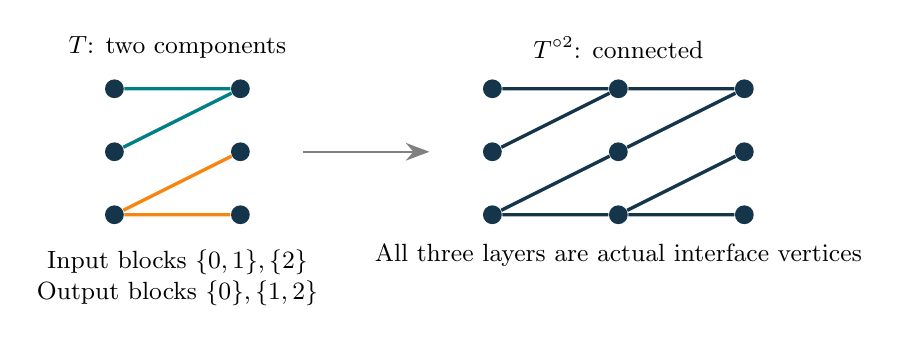
\begin{tikzpicture}[scale=.8,vertex/.style={circle,fill=Ink,inner sep=2.4pt},
 every node/.style={font=\small}]
\foreach \y in {0,1,2}{
 \node[vertex] (a\y) at (0,-\y) {};
 \node[vertex] (b\y) at (2,-\y) {};
 \node[vertex] (c\y) at (6,-\y) {};
 \node[vertex] (d\y) at (8,-\y) {};
 \node[vertex] (e\y) at (10,-\y) {};
}
\draw[Accent,very thick] (a0)--(b0) (a1)--(b0);
\draw[BurntOrange,very thick] (a2)--(b1) (a2)--(b2);
\draw[Ink,very thick] (c0)--(d0) (c1)--(d0) (c2)--(d1) (c2)--(d2)
 (d0)--(e0) (d1)--(e0) (d2)--(e1) (d2)--(e2);
\draw[-{Stealth[length=3mm]},gray,thick] (3,-1)--(5,-1);
\node at (1,.65) {$T$: two components};
\node at (8,.65) {$T^{\circ2}$: connected};
\node[align=center] at (1,-3) {Input blocks $\{0,1\},\{2\}$\\
Output blocks $\{0\},\{1,2\}$};
\node at (8,-2.65) {All three layers are actual interface vertices};
\end{tikzpicture}
\caption{A through tile with initially different component partitions.
After two copies the graph is connected and hence aligned. This diagram
illustrates exact reblocking only; it is not a cubic terminal pattern.}
\label{fig:reblocking}
\end{figure}

\subsection{Large binary graph examples}

The aligned star--triangle tile has seven vertices and six edges, interfaces
$L=(0,1,2)$ and $R=(3,4,5)$, and edge list
\[
 (0,6),(4,6),(5,6),(1,2),(2,3),(3,1).
\]
Its star component transports one input port to two output ports; its
triangle component transports the two remaining input ports to one output.
The induced component permutation is a transposition. Its closed $N$-copy
graph has $4N$ vertices and $6N$ edges. At $N=1$ it is $K_4$, supplying a
positive finite graph certificate. At odd large $N$, the routed kernel has
36 vertices and 54 edges. For $N=2^{4096}+1$, the retained proof lifts its
negative query answer without enumerating any missing copies.

The misaligned through example also uses $N=2^{4096}+1$, but needs an
exact reblocking period of two first. It produces a 54-vertex, 81-edge kernel.
Its source and formatted certificate occupy 1,806 and 11,384 bytes,
respectively. A three-edge cut includes an original edge at copy $N-1$,
which tests the nonzero-tail address formula rather than only an early
retained copy. Five source-production-plus-replay samples have median
1.519 milliseconds. This is a local binary-input demonstration; the
prototype has not constructed a corresponding native knot hierarchy.

For an illustration of the avoided global period, use permutation cycles
of lengths
\[
 2,3,5,7,11,13,17,19,23,29,31,37,41,43,47,53,59,61,67,71.
\]
The width is 639 and their global order is
$557940830126698960967415390$. At exponent $2^{2048}+12345$, componentwise
construction writes 132,226 vertices and 131,587 edges in 0.249 seconds in
the retained run. It never writes that global order as a word. This example
uses matching components and has degree two after closure; it tests only
the general graph-kernel construction and makes no cubic terminal verdict.

\subsection{Paired graph-query performance}

Both timed arms construct their graph, answer the same cubic marked-cut
predicate with the same finite certificate engine, and replay a certificate.
The explicit arm expands the entire source. The routed arm constructs the
bounded kernel and additionally replays its source reduction. Parsing,
serialization, sphere and ball validation, and knot recognition are outside
both timers. Each case has a warmup and seven paired rounds with shuffled
arm order; garbage collection occurs outside each timer. The final routing
run followed completion of the other in-session benchmark jobs.

\begin{center}\small
\begin{tabular}{rrrrrr}
\toprule
Copies & Original edges & Kernel edges & Explicit (ms) & Routed (ms) & Paired ratio\\
\midrule
1 & 6 & 6 & 0.108 & 0.208 & 0.53\\
3 & 18 & 18 & 0.059 & 0.241 & 0.25\\
9 & 54 & 54 & 0.103 & 0.380 & 0.27\\
33 & 198 & 54 & 0.268 & 0.395 & 0.66\\
129 & 774 & 54 & 1.023 & 0.363 & 2.86\\
513 & 3,078 & 54 & 4.281 & 0.377 & 11.04\\
2,049 & 12,294 & 54 & 17.616 & 0.421 & 42.97\\
8,193 & 49,158 & 54 & 80.700 & 0.459 & 198.94\\
\bottomrule
\end{tabular}\end{center}


Times are separate medians; ``paired ratio'' is the median of the seven
within-round explicit/routed ratios, so it need not equal the ratio of the
two displayed medians. The identical-explicit A/A control at 129 copies has
paired median ratio 1.009. The one-, three-, nine-, and thirty-three-copy
cases expose genuine reduction overhead. At 8,193 copies, the explicit
median is 80.700 milliseconds and the routed median is 0.459 milliseconds.
The family has a quickly found negative cut at the larger sizes; this is
a complete local graph query, not a worst-case positive-flow benchmark or a
comparison with the fastest possible cubic-connectivity implementation.

For exponent lengths $65,257,1025,4097,16385$ bits, the same aligned
54-edge kernel has retained query-plus-replay medians
$0.293,0.277,0.305,0.414,0.610$ milliseconds. The corresponding compact
JSON certificate sizes are $1768,1960,2728,5800,18088$ bytes under this
benchmark's serialization. Graph size is constant in that experiment;
arithmetic, source binding, and certificate size still depend on exponent
bit length. The source and certificate formatting for the separate through
example is different and should not be compared byte-for-byte as an
algorithmic compression ratio.

\begin{figure}[tb]
\centering
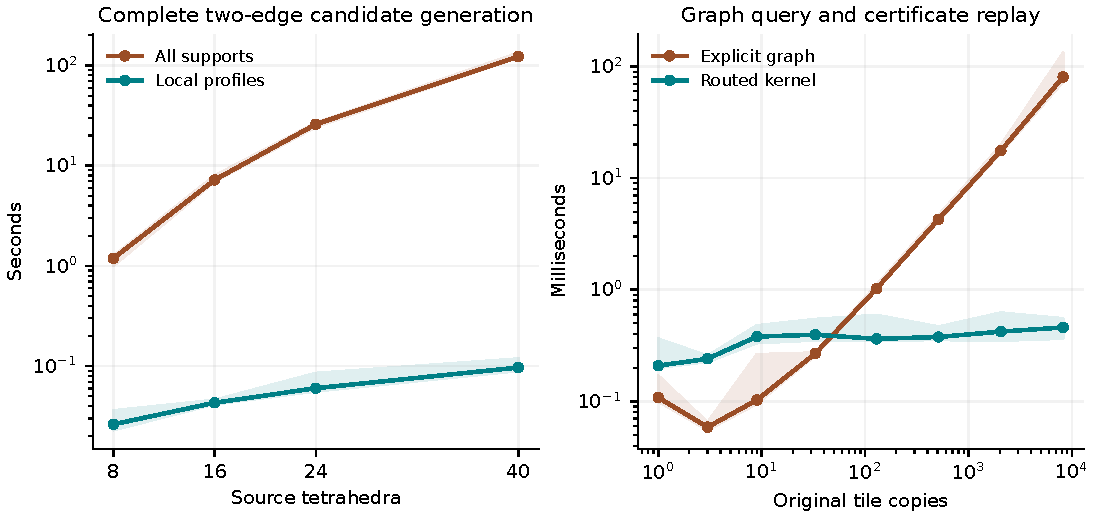
\includegraphics[width=\linewidth]{figures/performance.pdf}
\caption{Two distinct local performance comparisons. Lines show retained
medians and shading shows the observed sample ranges. Left: complete
radius-two candidate generation on the layered obstruction family, with
equal candidate sets and no topology-gate timing. Right: graph construction,
query, and certificate replay on the star--triangle family. These measurements
do not establish an end-to-end asymptotic knot-recognition bound.}
\label{fig:performance}
\end{figure}

\subsection{Interpretation and limitations of the measurements}

The strongest measured search gain is in exhaustive multi-edge candidate
generation. The clearest geometric gain is additional completed native
classifications. The graph gain removes numerical multiplicity from a query
whose faithful source grammar is already supplied. These are different
improvements and cannot be multiplied to obtain a claimed recognition speedup.

All timings come from one shared execution environment and small deliberately
specified families. Raw rounds and ranges are retained; no hardware-isolation
claim is made. The proofs establish the stated asymptotic reductions under
their hypotheses. The experiments establish agreement, rejection behavior,
source lifting, and the local costs actually measured. A broader native
workload is needed to decide the dispatch policy and identify which remaining
geometric interface dominates a complete run.

\section{What would suffice for a quasi-polynomial recognizer}
\label{sec:global-budget}

\subsection{An explicit parameter target for disc discovery}

The logarithm of the bound in Theorem~\ref{thm:cluster-complexity} is, up to
fixed additive polynomial terms,
\[
 r\log t+k\log(Cd^2)+O\bigl(\log t+\log(k+1)+\log(B+1)\bigr).
\]
This expression is more useful than a single claim that cancellation should
be small. It identifies two different geometric questions: how dispersed the
defects are, and how densely their edges meet tetrahedra.

\begin{corollary}[A sufficient discovery budget]\label{cor:discovery-budget}
Suppose the encoded source sizes, coherent-coordinate bit lengths, and
parameter budgets are polynomial in an original input size $n$. If a promised
vertex meridian satisfies
\[
 r\log(n+1)+k\log(d+1)=O\bigl((\log(n+1))^2\bigr),
\]
then the complete cancellation-cluster search on that source is bounded by
$n^{O(\log n)}$ bit operations.
\end{corollary}
\begin{proof}
Use $t\leq n^{O(1)}$ in the displayed logarithmic bound. Since $d\geq1$,
$k\log(Cd^2)=O(k\log(d+1))$ for the fixed positive constant $C$. The
remaining polynomial factors contribute $O(\log n)$ to the logarithm.
\end{proof}

For bounded $d$, the sufficient region includes
$r=O(\log n)$ and $k=O((\log n)^2)$. For
$d\leq(\log n)^A$ it includes
$k=O((\log n)^2/\log\log(n+2))$ with the same $r$ bound.
For $d=\Theta(n)$ it requires $r+k=O(\log n)$ in this estimate. With
bounded $d$ and fixed $r$, even $k=O(\log n)$ yields polynomial discovery.
These are conditional consequences of a proved local algorithm. No source
transformation controlling these parameters on all unknot inputs is supplied.

\subsection{Accounting for branching, failed attempts, and repairs}

A short successful hierarchy does not bound an algorithm that searches many
unsuccessful ones. The following elementary counting lemma supplies a precise
way to state the missing obligation. It applies to an actual execution tree,
including unsuccessful candidate choices and corrective operations.

\begin{lemma}[Branch-budget accounting]\label{lem:branch-budget}
Let a finite rooted execution tree have height at most $H$. For each internal
vertex $v$, let $b(v)\geq1$ be its actual number of children. Suppose every
root-to-leaf path $P$ satisfies
\[
 \sum_{v\in P,\ v\text{ internal}}\log b(v)\leq R.
\]
The tree has at most $e^R$ leaves and at most $(H+1)e^R$ vertices.
If all work charged to any one vertex is at most $W$, total work is at most
$(H+1)e^R W$.
\end{lemma}
\begin{proof}
At every internal vertex choose a child uniformly. A leaf at path $P$ is
reached with probability $\prod_{v\in P}b(v)^{-1}\geq e^{-R}$. Leaf
probabilities sum to one, proving the leaf bound. Every vertex belongs to
some root-to-leaf path, each of length at most $H$, so counting the union of
these paths with multiplicity gives at most $(H+1)$ times the number of
leaves. The last assertion follows by summing the work charges.
\end{proof}

The height condition controls arbitrarily long unary runs. The branch sum
controls actual alternatives, including abandoned choices. A restart or
repair must either appear in this execution tree or have its separate cost
explicitly charged. A potential that decreases only on the final successful
path does not satisfy this requirement.

For example, a complete faithful implementation would meet the stronger
quasi-polynomial target if it proved all of the following jointly:
\begin{enumerate}
\item Every reached source and all transported objects have polynomial
encoded size, and every surface-search call is complete for its required
topological task under the discovery budget above.
\item Every expensive terminal pattern query has a polynomial-size faithful
flat descriptor whose tiles are through, or is handled by another proved
operation with the same cost bound.
\item Bundle extraction, core certification, every remaining saturated
attachment, and curve/disc transport take at most $n^{O(\log n)}$ work per
execution node, including their certificate replay.
\item The complete execution, including failure, cleanup, and restart nodes,
has $H\leq n^{O(1)}$ and $R=O((\log n)^2)$.
\end{enumerate}
The local results in this report replace concrete terms in this list.
Lemma~\ref{lem:branch-budget} then combines the terms. The list is a research
contract, not a theorem that the present recognizer already satisfies it.

\subsection{The residual geometry after free-boundary condensation}

The unsaturated theorem removes all new relations coming from a proper
vertical attachment. Among attached bordered bases, if $\sigma$ are saturated,
there exists a relative decomposition with exactly $\sigma$ additional
two-handles from those bases.
This suggests measuring complexity by a residual attaching system rather than
by numerical genus or the number of product handles. It also gives a sharper
diagnostic: a failure in an unsaturated region should be a source-chart or
core-certification issue, or a resource limit, for the unmarked census. New
relations from these attachments occur in the saturated residue. Marked
transport remains a separate issue even on an unsaturated base.

Relator count alone is insufficient. A single attaching curve can be long,
can interact with many core handles, and must remain embedded with its source
framing. A useful next reduction would output a small triangulated marked core
and compressed boundary curves, together with a proof of their geometric
meaning. The source-parallelity $30t$ bound is linear in the current source;
it supplies neither a polylogarithmic residual core nor short transported
attaching words automatically.

There is already a relevant algorithmic result: Chambers, Lazarus, de Mesmay,
and Parsa decide contractibility of a compressed boundary curve in a
triangulated three-manifold in time
$2^{O(s^3)}\poly(L)$, where $s$ is the triangulation size and $L$ is the
compressed curve description size \cite{compressed-contractibility}.
Thus, if a future certified reduction gave a residual triangulation with
$s=O(\log n)$ and $L\leq n^{O(1)}$, this existing theorem would yield
$n^{O((\log n)^2)}$ for that contractibility task. For
$s=O((\log n)^{2/3})$ it would yield the stronger $n^{O(\log n)}$ bound.
This is an algebraic substitution into a published theorem, not a new
contractibility algorithm. It also concerns one specified task; finding all
needed curves and recognizing the resulting manifold require additional work.

\subsection{Why the pattern result changes the remaining target}

The incoming disconnected-pattern question required control of a potentially
large global permutation order. Componentwise routing removes that order.
Reblocking removes the need for initially aligned partitions whenever every
component meets both interfaces. Consequently a faithful flat through-tile
descriptor is now sufficient; there is no need to force every original tile
to be connected or to have logarithmic interface width.

This enlarges the target class for a geometric producer in a precise way.
The remaining obstructions are components missing an interface, access to
private tile vertices by later geometry, and unrestricted nested reuse.
These are concrete structural properties that can be logged at the native
pattern-transport boundary. Measuring those failures is more informative than
inferring applicability from a large numerical parallelity multiplicity alone.

\section{Further research questions and a proposed program}
\label{sec:research-program}

The results suggest a research program centered on geometric interfaces and
explicit parameter budgets. The priorities below are ordered by their ability
to connect the proved local reductions to a complete recognition procedure.
Each asks for a mathematical statement or a reproducible artifact that can be
accepted or falsified independently.

\subsection{Priority I: close the native geometric interfaces}

\paragraph{1. A faithful through-tile producer.}
Can the source-parallelity charts and ordered cut-boundary words produce a
flat descriptor of the actual transported cubic pattern in polynomial encoded
time? The new theorem allows disconnected tiles and initially different
component partitions. A first target is a nontrivial complete class of normal
cuts with a proof that every tile component meets both interfaces. The producer
must record the spherical embedding, actual port identities, edge ownership,
and why subsequent context has no access to private vertices. A useful
experiment logs these facts and each precise rejection reason on native
hierarchy cuts; a count of large multiplicities alone tests none of them.

\paragraph{2. Compressed relative bands with marked transport.}
Can the proper-boundary handle theorem be made constructive at the level of
source charts without writing one band per unit of genus? Seek a compressed
relative spine whose expansion gives the actual band system and whose actions
on ordered boundary arcs are polynomial in the encoded input. One should
specify which operations on that spine remain polynomial: intersection,
concatenation, extraction of a co-core disc, and transport of a boundary
pattern. A scalar genus counter settles the unmarked census but is insufficient
for any operation that must return an embedded curve or disc.

\paragraph{3. Compile the saturated residue geometrically.}
Each saturated bordered base contributes one two-handle in a suitable relative
decomposition. Can its attaching curve be encoded directly from the ordered
interface words and bundle charts, with a short embedded certificate? A
natural first family is planar saturated bases with a bounded number of
interfaces, followed by orientable bases with large binary genus and then
nonorientable bases. The output must preserve the attaching map and framing;
recording only its abelianization loses the distinction exhibited by
$\langle x,y\mid x^3=y^2\rangle$. A successful theorem should bound both
the number of residual curves and their encoded interaction with the core.

\paragraph{4. Extract a source-addressed geometric noose.}
The graph kernel gives at most three original crossing edges and a compressed
shore coloring. Can the actual spherical embedding turn this into a simple
closed curve with a compressed isotopy certificate, then transport the
corresponding disc through the hierarchy? This is an appropriate use of
existing efficient algorithms for curves on surfaces
\cite{lackenby-curves}. The extra issue is the source provenance linking those
surface calculations to the three-dimensional cut and its successive boundary
identifications. The first deliverable should cover a repeated native product
region, including reversed charts and corners.

\subsection{Priority II: prove discovery and execution budgets}

\paragraph{5. Bound the cancellation component count on useful sources.}
The fifteen-tetrahedron example proves that a one-component assumption cannot
be imposed on every vertex meridian. Does some broader small bound hold after
a certified source transformation, or can one construct a family in which the
minimum possible component count tends to infinity? A convincing negative
family must control \emph{all} vertex meridians, rather than exhibit one
complicated meridian. A positive theorem should bound the expression
$r\log n+k\log(d+1)$, which is what the discovery algorithm actually pays.
This is a more flexible target than independently minimizing all three
parameters.

\paragraph{6. Control incidence without losing the one-vertex model.}
Can certified moves reduce the maximum tetrahedron-incidence degree $d$ while
keeping $t$ and the required cancellation budget under control? Subdivision
can lower local incidence in some representations but may introduce vertices;
the fixed-cocycle proof then stops applying. The desired statement must
quantify this tradeoff and preserve the marked exterior. A useful intermediate
theorem would bound the sum of local profile costs over all affected
tetrahedron stars after a Pachner move, rather than restart every profile
search on the whole source.

\paragraph{7. Several vertices with shared potentials.}
For multiple vertices, write a representative as $c+\delta\phi$ and account
for the sign chambers of its edge values. Can local cancellation profiles be
coupled through a small exact system in the shared vertex potentials? A
Schur-complement or arrangement-based approach is plausible when the number
of independent potentials is small. The proof must retain integer feasibility
and the correct boundary-cohomology quotient. A real-valued local solution or
an arbitrary fixed vector $|c|$ would not be a complete substitute. The earlier
sign-chamber machinery provides a baseline against which a new bound should
be compared \cite{incoming-cancellation}.

\paragraph{8. Reduce the active-system dependence on incidence.}
The factor $(Cd^2)^k$ counts connected supports and then local active
hyperplane choices. Could these two enumerations be combined through an
incidence graph of equations and edges? A potential gain is a smaller
dependence on $d$ or a bound in the number of distinct local coefficient
patterns. The difficulty is that an active-system incidence graph can
disconnect even when the cancellation support is connected. Any pruning rule
must retain all extremal profiles, including the homogeneous exceptional
case; the current complete algorithm is an exact oracle for small tests.

\paragraph{9. Independently certify restricted exhaustion.}
The positive rank gate is compact. A general negative search transcript is
not yet supplied. Can one certify that every connected support and every
relevant active system up to the chosen budgets has been accounted for,
sharing repeated coefficient patterns and exact row reductions? The one-edge
inventory for the retained counterexample is a tractable starting case.
Such a transcript would establish exhaustion of a \emph{restricted} disc
class. It would become a nontriviality certificate only after a separate
theorem makes that class sufficient for all required meridians.

\paragraph{10. An amortized hierarchy potential for all work.}
Which geometric potential bounds both useful cuts and corrective operations,
while a branch budget controls all alternatives actually explored? A candidate
must be tested against source rebuilding, pattern normalization, saturated
repairs, and failed discovery. The execution-tree statement in
Lemma~\ref{lem:branch-budget} provides an explicit acceptance criterion.
Instrumenting these charges is useful before proving a global bound: a local
strict descent that triggers expensive unrestricted restarts may have little
practical value despite its mathematical validity.

\subsection{Priority III: enlarge and improve the graph kernels}

\paragraph{11. Tiles with births, deaths, and private components.}
The through hypothesis excludes a component that meets only one interface or
neither. Is there a polynomial marked-cut kernel for every binary tile power
at a fixed threshold? One possible route uses the larger partition-diagram
semigroup and records components that become internal during composition.
Purely private repeated connected components need only a bounded number of
representatives to supply the two marks, but components that enter and later
leave a through region require a source-addressed transient analysis. A proof
must track those components; the rank recurrence of
Lemma~\ref{lem:through-stabilization} deliberately does not cover them.

\paragraph{12. Can the quadratic reblocking bound be reduced?}
The exponent bound $m\leq d$ and the universal connected cutoff are sharp.
They do not show that a $d^2Q$ kernel is necessary. The sharper estimate
$(a_k+1)\sum_{\mathcal O}h_{\mathcal O}Q_{\mathcal O}+(m-1)Q$ already
distinguishes easy instances. Can shared cycle structure give an $O(Q)$ or
$O(Q\log Q)$ explicit marked representative, or is a superlinear lower bound
forced by exact boundary marks and source lifting? Known terminal mimicking
networks suggest comparison tools \cite{chalermsook2021,liu2023}, but their
construction from an expanded graph does not by itself solve the compressed
input problem.

\paragraph{13. Stable kernels under nested descriptions.}
Flat powers have explicit tiles. A general straight-line grammar may duplicate
already compressed subgraphs, so repeated local kernelization can increase
intermediate size. Identify a grammar class closed under the required
geometric operations for which kernel size is bounded by a fixed polynomial
in the whole grammar. A useful first result would charge each original edge
definition only a logarithmic number of times. The proof must preserve exposed
vertex identity and exact mark unions at each composition, not only the final
yes/no answer.

\paragraph{14. Smaller positive graph proofs.}
The dense replay path intentionally makes a conservative quartic pass over
the finite kernel. A sparse replay can remove an avoidable factor, and
positive anchor-pair proofs may share cut or flow structure. The mathematical
question is whether a short family of certified witnesses implies coverage
of all anchor pairs without enumerating them individually. The practical
question is where that proof work dominates source construction on native
patterns. Changes should be measured on complete producer-plus-replay queries,
including small instances where reduction overhead loses.

\subsection{A concrete sequence of research deliverables}

\begin{enumerate}
\item \textbf{Native interface census.} Instrument a fixed corpus of actual
hierarchy cuts. Record $(t,k,r,d)$ where measurable, saturated versus proper
base attachments, faithful tile sizes, through failures, and all source and
replay costs. Retain inconclusive outcomes and exact source identities.
\item \textbf{One complete geometric adapter.} Choose the largest clearly
specified family in that census for which a faithful pattern grammar and
relative band transport can both be proved. Deliver a source-bound producer
and independent replay, then measure completed recognition stages.
\item \textbf{One global parameter theorem or obstruction family.} Establish
a sufficient discovery budget on a certified family, or construct a family
forcing its violation. Either result would materially refine the strategy;
more favorable timings without such structural information would not.
\item \textbf{A complete execution account.} Integrate the proved adapters
with the maintained recognizer, charge every failed attempt and repair, and
state the final complexity theorem with all input-size conversions. Until
that account is complete, retain the local results as proved reductions and
their global use as an explicit research objective.
\end{enumerate}

\appendix
\section{Reproduction, dependency provenance, and file inventory}

The archive is self-contained for the three standard-library prototype suites
and the retained certificate replays. Run from its root:
\begin{verbatim}
python3 verify_all.py
PYTHONPATH=code python3 -m routed_patterns \
  examples/through_4097_bits.json --through \
  --output reproduced_through_certificate.json
PYTHONPATH=code python3 -m routed_patterns \
  examples/through_4097_bits.json \
  --verify examples/through_4097_bits_certificate.json
python3 experiments/reblocking_partition_audit.py \
  --max-width 5 --output results/repeated_partition_audit.json
python3 experiments/connected_cutoff_audit.py
cd article
latexmk -pdf -interaction=nonstopmode hierarchy_kernels.tex
\end{verbatim}

The verification runner isolates the three import environments, so the
different incoming dependency snapshots cannot accidentally replace one
another. It records the observed test counts and all saved-certificate
replays. The cancellation package defaults to its bundled runtime; environment
overrides can instead point to an explicitly prepared repository checkout.
The geometry package contains only its pinned transitive upstream modules and
the retained corpus, plus minimal reproduction package namespaces.

The recorded interpreter is CPython 3.12.14 on Linux x86-64. The production
code uses exact integers and rational arithmetic from the standard library.
Regina 7.4 is optional for the expanded geometric and full vertex-enumeration
oracles \cite{regina}; it is not needed for replaying the retained positive
certificates. Matplotlib is used only to regenerate the report's static
performance figure. The article builds with pdf\LaTeX\ and ordinary TeX Live
packages. Long full-enumeration benchmarks are separate from the quick
verification command and should be run without simultaneous compute-heavy
jobs.

\begin{longtable}{@{}>{\raggedright\arraybackslash}p{0.40\linewidth}
>{\raggedright\arraybackslash}p{0.55\linewidth}@{}}
\toprule
Path & Role\\\midrule\endhead
\path{article/hierarchy_kernels.tex}, \path{article/sections/} & Main article,
complete theorem proofs, experiment interpretation, and research program\\
\path{article/hierarchy_kernels.pdf} & Compiled and visually checked report\\
\path{article/connected_cutoff_supplement.tex} & Exact cutoff theorem and
sharp constructions at every threshold\\
\path{code/routed_patterns/} & New aligned routing, exact cutoff,
through-component reblocking, and independent checker\\
\path{code/pattern_kernel/} & Unchanged incoming tile types, finite graph
certificate engine, replay, and small full-signature oracle\\
\path{cancellation/fastunknot/} & New connected-profile discovery module and
unchanged incoming positive vertex-disc gate\\
\path{cancellation/runtime/} & Minimal pinned search dependencies and the
coherent-obstruction source fixture\\
\path{cancellation/artifacts/} & Exact disconnected disc, all external vertex
vectors, one-edge inventory, tests, and paired timing records\\
\path{geometry/code/unsaturated_bundles/} & Finite proper-boundary classifier,
independent census replay, and native source adapter\\
\path{geometry/vendor/}, \path{geometry/evidence/} & Pinned incoming runtime,
106-case corpus, five newly completed source certificates, and measurements\\
\path{examples/} & Four graph sources and independently replayable proofs,
including the large misaligned through-component example\\
\path{experiments/}, \path{results/} & Full-signature and partition audits,
source-coloring comparisons, timing drivers, raw results, and review records\\
\path{verify_all.py} & Quick isolated test and saved-certificate replay runner\\
\path{integration/INTEGRATION.md} & Additive repository placement and exact
native adapter contracts\\
\path{provenance/} & Source checkpoint and copied-dependency identities\\
\bottomrule
\end{longtable}

The archive deliberately includes enough pinned source to reproduce the
results without a live branch moving underneath them. Those copied modules
are not counted as new implementations. No maintained checkout changes,
remote repository writes, full native regression-suite run, or end-to-end
knot-recognition performance result is implied by this package.

\begin{thebibliography}{99}
\bibitem{repo}
Vladimir Reshetnikov and ProveIt contributors,
\emph{ProveIt: Topology/UnknotRecognition}, source revision
\texttt{a28a49ee5c4145db0facbeb1e7f65cd8a2816775}, 12 October 2026.
\url{https://github.com/VladimirReshetnikov/ProveIt/tree/a28a49ee5c4145db0facbeb1e7f65cd8a2816775/Topology/UnknotRecognition}.

\bibitem{repo-parallelity}
ProveIt contributors, \emph{Source parallelity bundles and inherited cores},
source manuscript \path{synthesis/parallelity.tex}, at the revision in [1].
\url{https://github.com/VladimirReshetnikov/ProveIt/blob/a28a49ee5c4145db0facbeb1e7f65cd8a2816775/Topology/UnknotRecognition/synthesis/parallelity.tex}.

\bibitem{incoming-cancellation}
ProveIt research continuation,
\emph{Sparse edge cancellation in unknot recognition: complete vertex-disc
search, explicit obstructions, and compressed boundary interfaces},
12 October 2026. Incoming archive
\path{docs/incoming/unknot_cancellation_20261012.zip};
main source \path{article/unknot_cancellation.tex}; exact edge-space prototype
\path{repro/Topology/UnknotRecognition/fast/fastunknot/normal_weight_defect.py};
positive gate \path{artifacts/edge_discovery/vertex_gate.py}.

\bibitem{incoming-reductions}
ProveIt research continuation,
\emph{Certified support and attachment-preserving product reductions for
unknot recognition}, 12 October 2026. Incoming archive
\path{docs/incoming/unknot_reductions_20261012.zip}.

\bibitem{incoming-marked}
ProveIt research continuation, \emph{Marked Parallelity Interfaces and Certified
Handlebody Cores: polynomial local topology and exact sector decomposition
for the unknot-recognition programme}, 12 October 2026. Incoming archive
\path{docs/incoming/ProveIt_Unknot_Marked_Parallelity_2026-10-12.zip};
main source \path{article.tex}; pinned runtime and 106-case source corpus
identified in this package's dependency provenance.

\bibitem{incoming-homology}
ProveIt research continuation,
\emph{Bounded-interface integral homology: binary surface condensation,
twisted attachments, and provenance-aware terminals for compressed unknot
hierarchies}, 12 October 2026. Incoming archive
\path{docs/incoming/ProveIt_Unknot_Interface_Homology_2026-10-12.zip}.

\bibitem{incoming-corners}
ProveIt research continuation, \emph{Corner-Aware Boundary Kernels for
Compressed Unknot Hierarchies: exact port surgery, orbit-count compilation,
and interval-bundle consequences}, 12 October 2026. Incoming archive
\path{docs/incoming/ProveIt_Corner_Aware_Boundary_Kernels_2026-10-12.zip}.

\bibitem{lackenby2026}
Marc Lackenby, \emph{Incompressible surfaces, hierarchies and unknot
recognition}, preprint, 25 July 2026, arXiv:2607.23350.
\url{https://arxiv.org/abs/2607.23350}.
Author's PDF:
\url{https://people.maths.ox.ac.uk/lackenby/algorithm-incompressible-250726.pdf}.

\bibitem{lackenby-talk}
Marc Lackenby, \emph{Unknot recognition in quasi-polynomial time},
lecture slides, February 2021.
\url{https://people.maths.ox.ac.uk/lackenby/quasipolynomial-talk.pdf}.
The announcement and the later detailed preprint are distinct source types.

\bibitem{aht}
Ian Agol, Joel Hass, and William Thurston,
\emph{The Computational Complexity of Knot Genus and Spanning Area},
Transactions of the American Mathematical Society \textbf{358}(9) (2006),
3821--3850. Preprint: \url{https://arxiv.org/abs/math/0205057}.

\bibitem{lackenby-curves}
Marc Lackenby, \emph{Some Fast Algorithms for Curves in Surfaces},
Discrete \& Computational Geometry \textbf{76} (2026), 539--588.
\url{https://doi.org/10.1007/s00454-026-00845-7}.

\bibitem{compressed-contractibility}
Erin W. Chambers, Francis Lazarus, Arnaud de Mesmay, and Salman Parsa,
\emph{Algorithms for Contractibility of Compressed Curves on 3-Manifold
Boundaries}, Discrete \& Computational Geometry \textbf{70} (2023),
323--354. \url{https://doi.org/10.1007/s00454-022-00411-x}.
Preprint: \url{https://arxiv.org/abs/2012.02352}.

\bibitem{regina}
Benjamin A. Burton and the Regina development team,
\emph{Regina: Software for low-dimensional topology}, version 7.4,
used for the optional independent finite normal-surface and cut-manifold
audits in this report. \url{https://regina-normal.github.io/}.
The production reductions and certificate replay use Python's standard library.


\bibitem{incoming-four-copy}
ProveIt research continuation,
\emph{Four-Copy Kernels for Compressed Boundary Patterns:
Marked cut signatures, sharp repetition bounds, and certified terminal tests
for unknot hierarchies}, 12 October 2026.
Incoming research package, file
\texttt{article/four\_copy\_patterns.tex};
Theorems on connected repetition and four-copy equivalence.

\bibitem{hagerup1998}
Torben Hagerup, Jyrki Katajainen, Naomi Nishimura, and Prabhakar Ragde,
\emph{Characterizing Multiterminal Flow Networks and Computing Flows in
Networks of Small Treewidth},
Journal of Computer and System Sciences \textbf{57}(3) (1998), 366--375.
\url{https://doi.org/10.1006/jcss.1998.1592}.

\bibitem{chalermsook2021}
Parinya Chalermsook, Syamantak Das, Bundit Laekhanukit, Yunbum Kook,
Yang P. Liu, Richard Peng, Mark Sellke, and Daniel Vaz,
\emph{Vertex Sparsification for Edge Connectivity},
Proceedings of the 2021 ACM--SIAM Symposium on Discrete Algorithms
(SODA 2021), 1206--1225.
\url{https://doi.org/10.1137/1.9781611976465.74}.
Preprint: \url{https://arxiv.org/abs/2007.07862}.

\bibitem{liu2023}
Yang P. Liu,
\emph{Vertex Sparsification for Edge Connectivity in Polynomial Time},
14th Innovations in Theoretical Computer Science Conference (ITCS 2023),
Leibniz International Proceedings in Informatics \textbf{251},
83:1--83:15 (2023).
\url{https://doi.org/10.4230/LIPIcs.ITCS.2023.83}.
Preprint: \url{https://arxiv.org/abs/2011.15101}.


\bibitem{fitzgerald-leech1998}
D.~G.~FitzGerald and Jonathan Leech,
\emph{Dual symmetric inverse monoids and representation theory},
Journal of the Australian Mathematical Society, Series A,
\textbf{64} (1998), 345--367.
\url{https://doi.org/10.1017/S1446788700039227}.

\bibitem{easdown-east-fitzgerald2008}
David Easdown, James East, and D.~G.~FitzGerald,
\emph{A presentation of the dual symmetric inverse monoid},
International Journal of Algebra and Computation \textbf{18}(2) (2008),
357--374.
\url{https://doi.org/10.1142/S0218196708004470}.
Preprint: \url{https://arxiv.org/abs/0707.2439}.

\end{thebibliography}
\end{document}
